\begin{enumerate}[label=\thechapter.\arabic*,ref=\thechapter.\theenumi]
\item The network shown below has a resonant frequency of 150 kHz and bandwidth of 600
Hz. The Q-factor of the network is \rule{1cm}{0.15mm}\\
(rounded off to one decimal place).\\
\hfill(GATE 2022 EC)\\
\begin{figure}[ht]
  \centering
  
      \begin{circuitikz}[american]
   \draw (0,8) to [sV=200V](0,-1) to [short](6,-1) to [short](6,0) to [D,l=$D_3$](9,3);
   \draw (0,8) to [short](6,8) to [short](6,6);
   \draw (6,6) to [D,l=$D_1$](9,3);
   \draw (3,3) to [D,l=$D_4$](6,6);
   \draw (3,3) to [D,l=$D_2$](6,0);
   \draw (3,3) to [short](2.5,3) to [crossing, bipoles/crossing/size=1](2.5,-4.8) to [short](12,-4.8) to [R=50$\Omega$](12,3) to [short](9,3);
   \draw (9,3) to [short,i=\Large{I}](12,3);
\end{circuitikz}

  
  \caption{Circuit 1}
\end{figure}\\
\solution\\
 \iffalse
\let\negmedspace\undefined
\let\negthickspace\undefined
\documentclass[journal,12pt,onecolumn]{IEEEtran}
\usepackage{cite}
\usepackage{amsmath,amssymb,amsfonts,amsthm}
\usepackage{algorithmic}
\usepackage{graphicx}
\usepackage{textcomp}
\usepackage{xcolor}
\usepackage{txfonts}
\usepackage{listings}
\usepackage{enumitem}
\usepackage{mathtools}
\usepackage{gensymb}
\usepackage{comment}
\usepackage[breaklinks=true]{hyperref}
\usepackage{tkz-euclide} 
\usepackage{tikz}
\usepackage{circuitikz}
%\usetikzlibrary{circuits.ee.IEC}
\usepackage{listings}
\usepackage{gvv} 
\usepackage{caption}
\def\inputGnumericTable{}                   

%\usepackage[latin1]{inputenc}                                
\usepackage{color}                                            
\usepackage{array}                                            
\usepackage{longtable}                                       
\usepackage{calc}                                             
\usepackage{multirow}                                         
\usepackage{hhline}                                           
\usepackage{ifthen}                                           
\usepackage{lscape}
\usepackage{tikz}
\usepackage{circuitikz}

\newtheorem{theorem}{Theorem}[section]
\newtheorem{problem}{Problem}
\newtheorem{proposition}{Proposition}[section]
\newtheorem{lemma}{Lemma}[section]
\newtheorem{corollary}[theorem]{Corollary}
\newtheorem{example}{Example}[section]
\newtheorem{definition}[problem]{Definition}
\newcommand{\BEQA}{\begin{eqnarray}}
\newcommand{\EEQA}{\end{eqnarray}}
\newcommand{\define}{\stackrel{\triangle}{=}}
\theoremstyle{remark}
\newtheorem{rem}{Remark}

\begin{document}

\bibliographystyle{IEEEtran}
\vspace{3cm}

\title{GATE: EE - 59.2022}
\author{EE23BTECH11013 - Avyaaz$^{*}$% <-this % stops a space 
}
\maketitle
% \newpage
% \bigskip

\renewcommand{\thefigure}{\arabic{figure}}
\renewcommand{\thetable}{\arabic{table}}

\large\textbf{\textsl{Question:}}
For the ideal AC-DC rectifier circuit shown in the figure below, the load current
magnitude is $I_{dc}$ = $15$ A and is ripple free. The thyristors are fired with a delay angle
of 45\degree
. The amplitude of the fundamental component of the source current, in
amperes, is \_\_\_\_\_\_\_\_{\em (Round off to 2
decimal places)}. \hfill(GATE 59 EE 2022)
\begin{figure}[!h]
\centering
\begin{circuitikz}[american voltages]
    \draw (0,0) node[op amp] (opamp) {};
    \draw (opamp.+) node[above]{$v_{+}$} to (-2,-0.5);
    \draw (opamp.-) node[above]{$v_{-}$} to (-2, 0.5);
    \draw (opamp.out) to (2, 0)node[right]{$v_{out}$};
    \draw (opamp.down) to (-0.1, -1) node[below]{$-v_{EE}$};
    \draw (opamp.up) to (-0.1, 1)node[above]{$+v_{DD}$};
    \draw (-2,0.5) to [R, l_=$R_1$](-3,0.5) to (-3.5, 0.5) to [V, l_=$0.1v$] (-3.5, -2) node[ground]{};
    \draw (-2, -0.5) to [R, l=$R_2$] (-2, -2) node[ground]{};
    \draw (-1.5,0.5) to (-1.5, 2) to [C, l=$C_1$] (1.5, 2) to (1.5, 0);
\end{circuitikz}

\end{figure}

\solution
\fi
\begin{table}[htbp]
\setlength{\extrarowheight}{4pt}
\setlength{\tabcolsep}{3pt}
\centering
\begin{tabular}{|c|c|c|}
\hline
\textbf{Parameter} & \textbf{Description}&\textbf{Value}\\
\hline 
$I_{dc}$& Load current & $15$A  \\
\hline
$\alpha$ &Firing angle&$45\degree$ \\
\hline
\end{tabular}

\caption{}
\label{tab:inputs.EE.59.2022}
\end{table}
% It is a Single phase symmetrical semi-converter.
% \begin{enumerate}[label={\roman*)}]
%     \item Load current magnitude $\brak{I_{dc}}$ = $15$A
%     \item Firing angle $\brak{\alpha} = 45\degree$
% \end{enumerate}
A symmetrical single phase semi converter is shown below,

\begin{figure}[!h]
\centering
    \begin{circuitikz}[scale = 0.8]
      \draw (-0.8,0.8) -- (-0.8,0.8) node[above]{$+$};
    \draw (0,2) to[sV,l=$V_s$] (0,-1);
     \draw (-0.8,0) -- (-0.8,0) node[below]{$-$};
    \draw (0,2) -- (2,2);
    \draw (2,2) -- (2,1);
    \draw (2,1) -- (3,1);
     \draw (3,1) to [thyristor] (3,3);
     \node at (2.4,2.3) {$T_1$};
    \draw (3,3) -- (5,3);
    \draw (5,1) to [thyristor] (5,3);
     \node at (4.4,2.3) {$T_2$};
    \draw (5,3) -- (7,3);
    \draw (7,3) to[resistor](7,1);
    \draw (7,1) -- (7,0);
    \draw(7,0) to [L](7,-2);
    \draw (7,-2) -- (3,-2);

    \draw (0, -1) -- (2,-1);
    \draw (2,-1) -- (2,0.4);
    \draw (2,0.4) -- (5,0.4);
    \draw (3,-2) to [Do] (3,0.4);
    \node at (3.8,-1) {$D_1$};
    \draw (3,0.4) -- (3,1);
    \draw (5,-2) to [Do] (5,0.4);
    \node at (5.8,-1) {$D_2$};
    \draw (5,0.4) -- (5,1);

     \draw[->] (6.5, 2) -- (6.5, 1) node[midway, left]{$I_{dc}$};
          \draw[->] (0.5, 2) -- (1, 2) ;
          \node at (1,1.6) {$I_s$};
          \node at (7.4,2) {$R$};
          \node at (7.4,-1.1) {$L$};

     \draw (8,2.8) -- (8,2.8) node[above]{$+$};
     \draw[->] (8,0.8) -- (8,2.8);
     \node at (8,0.5) {$V_o$};
     \draw[->] (8,0.2) -- (8,-1.8);
     \draw (8,-1.8) -- (8,-1.8) node[below]{$-$};
        \end{circuitikz}

\end{figure}

The Fourier series representation of supply current is given by:
\begin{align}
    i_s(t) = a_o +\sum_{n=1}^{\infty}C_n\sin({n\omega t} + \theta_n)\label{eq:gen_i_s}
\end{align}
 where,
 \begin{align}
 a_o &= \frac{1}{2\pi} \int_{0}^{2\pi} i_s(t)d\omega t \\
     C_n &= \sqrt{a_n^2 + b_n ^2}\label{eq:bino_coeff}\\
     \theta_n &= \tan^{-1}\left({\frac{a_n}{b_n}}\right)\label{eq: theta}
 \end{align}
\begin{align}
  \implies  a_o &= \frac{1}{2\pi}\int_{\alpha}^{\pi} I_o d\omega t - \int_{\pi + \alpha}^{2\pi} I_o d\omega t = 0\\
 \implies   a_n &= \frac{1}{\pi} \int_{\alpha}^{\pi}I_o\cos n\omega t d\omega t - \int_{\pi + \alpha}^{2\pi} I_o\cos{n\omega td\omega t}\\
 a_n &= 
 \begin{cases}
    \frac{-2I_o}{n\pi}\sin{n\alpha} & \text{for } n = 1,3,5...\\
     0 &\text{for } n = 2,4.....
    \end{cases}\\
 \implies   b_n &= \frac{1}{\pi}\int_{\alpha}^{\pi}I_o\sin n\omega t d\omega t - \int_{\pi + \alpha}^{2\pi} I_o\sin{n\omega td\omega t} \\
 b_n &= 
 \begin{cases}
     \frac{2I_o}{n\pi}\left(1 + \cos{n\alpha}\right) &\text{for } n = 1,3,5...\\
     0 &\text{for } n = 2, 4....
    \end{cases}
    \end{align}
From \eqref{eq:bino_coeff}:
\begin{align}
  \therefore  C_n &= \frac{2\sqrt{2}I_o}{n\pi}\left(\sqrt{1 + \cos{n\alpha}}\right)\\
  \implies  C_n &= \frac{4I_o}{n\pi}\cos{\frac{n\alpha}{2}}\label{eq:final_bino}
\end{align}
From \eqref{eq: theta}:
\begin{align}
    \theta_n &= \tan^{-1}\left(\frac{-\sin{n\alpha}}{1 + \cos{n\alpha}}\right)\\
    \implies \theta_n &= \frac{-n\alpha}{2}\label{eq:final_theta}
\end{align}

From \eqref{eq:gen_i_s},\eqref{eq:final_bino} and \eqref{eq:final_theta}:
\begin{align}
I_{s}(t) = \sum_{n=1,3,5...}^{\infty} \frac{4I_{o}}{n\pi}\cos{\frac{n\alpha}{2}}\sin{\left(n\omega t - \frac{n\alpha}{2}\right)}
\end{align}
% \begin{align}
% I_{s}(t) = \sum_{n=1,3,5...}^{\infty} \frac{4I_{dc}}{n\pi}\cos{\frac{n\alpha}{2}}\sin{\left(n\omega t - \frac{n\alpha}{2}\right)}
% \end{align}


% \begin{tikzpicture}[scale=1]
%     \draw[->] (0,0) -- (10,0) node[right] {$\omega t$};
%     \draw[->] (0,-2) -- (0,2) node[above] {$y$};
%     \draw[domain=0:10, smooth, variable=\x, black] plot ({\x},{sin(deg(\x))});
%     \foreach \x/\xtext in {1.57/\frac{\pi}{2},3.14/\pi,4.71/\frac{3\pi}{2},6.28/2\pi,7.85/\frac{7\pi}{2}} {
%         \draw (\x cm,0) -- (\x cm,0.1) node[below] {$\xtext$};
%     }
%     \foreach \y in {-1,1} {
%         \draw (1pt,\y cm-1.5) -- (-1pt,\y cm-1.5) node[left] {$\y$};
%     }
% \end{tikzpicture}

\begin{figure}[!h]
    \centering
    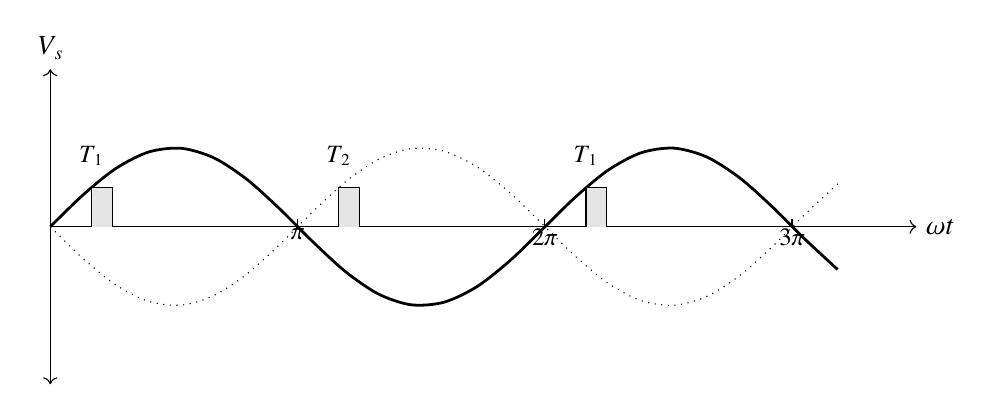
\begin{tikzpicture}[scale=1]
    \draw[->] (0,0) -- (11,0) node[right] {$\omega t$};
    \draw[<->] (0,-2) -- (0,2) node[above] {$V_s$};
    \draw[domain=0:10, smooth, variable=\x, black,line width=1pt] plot ({\x},{sin(deg(\x))});
    \draw[dotted,domain=0:10, smooth, variable=\x, black] plot ({\x},{-sin(deg(\x))});
    \foreach \x/\xtext in {3.14/\pi,6.28/2\pi,9.42/3\pi} {
        \draw (\x cm,0) -- (\x cm,0.1) node[below] {\small$\xtext$};
    }

\fill[gray!20] (0.5233,0) -- (0.5233,0.5) -- (0.785,0.5) -- (0.785,0) -- cycle;
    \fill[gray!20] (3.6633,0) -- (3.6633,0.5) -- (3.925,0.5) -- (3.925,0) -- cycle;
    \fill[gray!20] (6.8033,0) -- (6.8033,0.5) -- (7.065,0.5) -- (7.065,0) -- cycle;

    \draw (0.5233,0) -- (0.5233,0.5);
    \draw (0.5233,0.5) -- (0.785,0.5);
    \draw (0.785,0.5) -- (0.785,0);

    \draw (3.6633,0) -- (3.6633,0.5);
    \draw (3.6633,0.5) -- (3.925,0.5);
    \draw (3.925,0.5) -- (3.925,0);

    \draw (6.8033,0) -- (6.8033,0.5);
    \draw (6.8033,0.5) -- (7.065,0.5);
    \draw (7.065,0.5) -- (7.065,0);


     \node at (0.5233,0.9) {\small$T_1$};
     \node at (3.6633,0.9) {\small$T_2$};
     \node at (6.8033,0.9) {\small$T_1$};
\end{tikzpicture}
\end{figure}
\begin{figure}[!h]
    \centering
    \begin{tikzpicture}[scale=1]
    \draw[->] (0,0) -- (11,0) node[right] {$\omega t$};
    \draw[<->] (0,-2) -- (0,2) node[above] {$V_o$};
    \draw[domain=0.5233:3.14, smooth, variable=\x, black,line width=1pt] plot ({\x},{sin(deg(\x))});
    \draw[domain=3.6633:6.28, smooth, variable=\x, black,line width=1pt] plot ({\x},{-sin(deg(\x))});
    \draw[domain=6.8033:9.42, smooth, variable=\x, black,line width=1pt] plot ({\x},{sin(deg(\x))});

    \foreach \x/\xtext in {0.5233/\alpha, 3.14/\pi,4/\pi + \alpha ,6.28/2\pi,7.2/2\pi + \alpha,9.42/3\pi}{
        \draw (\x cm,0) -- (\x cm,0) node[below] {\small $\xtext$};
    }

     \draw [line width=1pt](0,0)--(0.5233,0);
    \draw [line width=1pt](0.5233,0) -- (0.5233,0.5);
    \draw[line width=1pt](3.14,0)-- (3.6633,0);
    \draw[line width=1pt] (3.6633,0) -- (3.6633,0.5);
    \draw [line width=1pt](6.28,0)--(6.8033,0);
    \draw [line width=1pt](6.8033,0) -- (6.8033,0.5);

    \node at (0.25,0.6){\small$T_2$};
    \node at (0.25,0.2){\small$D_2$};
     \node at (3.4,0.6){\small$T_1$};
    \node at (3.4,0.2){\small$D_1$};
    \node at (6.4,0.6){\small$T_2$};
    \node at (6.4,0.2){\small$D_2$};

    \node at (1.57,0.4){\small $T_1D_2$};
    \node at (4.71,0.4){\small $T_2D_1$};
    
\end{tikzpicture}
\end{figure}
\begin{figure}[!h]
    \centering
    \begin{tikzpicture}[scale=1]
    \draw[->] (0,0) -- (11,0) node[right] {$\omega t$};
    \draw[<->] (0,-2) -- (0,2) node[above] {$i_{T_1}$};
   
    \foreach \x/\xtext in {0.5233/\alpha,4/\pi + \alpha,7.2/2\pi + \alpha,10/3\pi + \alpha}{
        \draw (\x cm,0) -- (\x cm,0) node[below] {\small $\xtext$};
    }
     \draw [line width=1pt](0,0)--(0.5233,0);
    \draw [line width=1pt](0.5233,0) -- (0.5233,1);
    \draw[line width=1pt](0.5233,1)-- (3.6633,1);
    \draw[line width=1pt] (3.6633,1) -- (3.6633,0);
    \draw[line width=1pt] (3.6633,0) -- (6.8033,0);
    \draw [line width=1pt](6.8033,0)--(6.8033,1);
    \draw [line width=1pt](6.8033,1) -- (9.948,1);
     \draw [line width=1pt] (9.948,1) -- (9.948,0);

     \draw[dotted,domain=0:10, smooth, variable=\x, black] plot ({\x},{1});
     \node at (0.4,1.2) {\small $I_{DC}$};
\end{tikzpicture}
\end{figure}
\begin{figure}[!h]
    \centering
    \begin{tikzpicture}[scale=1]
    \draw[->] (0,0) -- (11,0) node[right] {$\omega t$};
    \draw[<->] (0,-2) -- (0,2) node[above] {$i_{s}$};
   

    \draw [line width=1pt](0.5233,0) -- (0.5233,1);
    \draw[line width=1pt](0.5233,1)-- (3.14,1);
    \draw[line width=1pt](3.14,1)-- (3.14,0);
    \draw[line width=1pt] (3.14,0) -- (3.6633,0);
    \draw[line width=1pt] (3.6633,0) -- (3.6633,-1);
    \draw[line width=1pt] (3.6633,-1) -- (6.28,-1);
    \draw[line width=1pt]  (6.28,-1) -- (6.28,0);
    \draw[line width=1pt] (6.28,0) -- (6.8033,0);
    \draw [line width=1pt](6.8033,0)--(6.8033,1);
    \draw [line width=1pt](6.8033,1) -- (9.42,1);
     \draw [line width=1pt] (9.42,1) -- (9.42,0);
     \draw [line width=1pt] (9.42,0) -- (9.948,0);

     \draw[dotted,domain=0:10, smooth, variable=\x, black] plot ({\x},{1});
     \node at (0.4,1.2) {\small $I_{DC}$};
    
\end{tikzpicture}
\end{figure}

From \tabref{tab:inputs.EE.59.2022}:
\begin{align}
   (I_{s_1})_{peak} &= \frac{4I_{dc}}{\pi}\cos{\left(\frac{\alpha}{2}\right)}\\
    &= \frac{4 \times 15 }{\pi}\times \cos{\frac{45 \degree}{2}}\\
    &=17.64 A 
\end{align}

%\end{document}

\pagebreak
\item A circuit with an ideal OPAMP is shown. The Bode plot for the magnitude (in dB)
 of the gain transfer function $ \brak{A \brak{j \omega}} = \dfrac{ V_{out}\brak{j \omega}}{V_{in}\brak{j \omega}}$ of the circuit is also
provided (here, $\omega$ is the angular frequency in $ rad/s $). The values of $R$ and $C$ are 
\begin{figure}[ht]
	\centering
    \includegraphics[width=\columnwidth]{2022/EC/42/figs/fig1.png}
    \label{fig:2022.42.39}
\end{figure} 
\begin{enumerate}[label = (\Alph*)]
     \item $R$ = $3k\ohm$,  $C$ = $1\mu F$\\
     \item $R$ = $1k\ohm$,  $C$ = $3\mu F$\\
     \item $R$ = $4k\ohm$,  $C$ = $1\mu F$\\
     \item $R$ = $3k\ohm$,  $C$ = $2\mu F$\\
\end{enumerate}
\hfill(GATE 2022 EC)\\
\solution\\
\input{2022/EC/42/ec.tex}
\pagebreak

\item  In the circuit shown, the load is driven by a sinusoidal A.C. voltage source $V_1 = 100\angle0\degree V$ at $50Hz$. Given $R_1 = 20\Omega$, $C_1 = \brak{\frac{1000}{\pi}}\mu F$, $L_1 = \brak{\frac{20}{\pi}}mH$ and $R_2 = 4\Omega$, the power factor is \_\_\_\_\_ (round off to one decimal place)\\
\hfill(GATE 2022 IN Q52)
\begin{figure}[!h]
    \centering
    \begin{circuitikz}
        \draw(0, 0) to[sV, l = $V_1$](0, -4);
        \draw(0, -4) to [R, l = $R_2$](6, -4);
        \draw(6, 0) to[L, l = $L_1$](6, -4);
        \draw(0, 0) -- (2, 0);
        \draw(4, 0) -- (6, 0);
        \draw(2, 0.75) -- (2, -0.75);
        \draw(4, 0.75) -- (4, -0.75);

        \draw(2, 0.75) to [R, l = $R_1$](4, 0.75);
        \draw(2, -0.75) to [C, l_ = $C_1$](4, -0.75);
    \end{circuitikz}
    \caption{}
    \label{fig:1_gate.22.in.52}
\end{figure}

\solution
\iffalse
\let\negmedspace\undefined
\let\negthickspace\undefined
\documentclass[journal,12pt,twocolumn]{IEEEtran}
\usepackage{cite}
\usepackage{amsmath,amssymb,amsfonts,amsthm}
\usepackage{algorithmic}
\usepackage{graphicx}
\usepackage{textcomp}
\usepackage{xcolor}
\usepackage{txfonts}
\usepackage{listings}
\usepackage{enumitem}
\usepackage{mathtools}
\usepackage{gensymb}
\usepackage{comment}
\usepackage[breaklinks=true]{hyperref}
\usepackage{tkz-euclide} 
\usepackage{listings}
\usepackage{gvv}                            \usepackage{tikz}
\usepackage{circuitikz}
\def\inputGnumericTable{}                                
\usepackage[latin1]{inputenc}                            
\usepackage{color}                      \usepackage{gensymb}
\usepackage{array}                                       
\usepackage{longtable}                                   
\usepackage{calc}                              
\usepackage{tikz}
\usepackage{multirow}                                    
\usepackage{hhline}                                      
\usepackage{ifthen}                            
\usepackage{caption}
\usepackage{lscape}
\usepackage{amsmath}
\newtheorem{theorem}{Theorem}[section]
\newtheorem{problem}{Problem}
\newtheorem{proposition}{Proposition}[section]
\newtheorem{lemma}{Lemma}[section]
\newtheorem{corollary}[theorem]{Corollary}
\newtheorem{example}{Example}[section]
\newtheorem{definition}[problem]{Definition}
\newcommand{\BEQA}{\begin{eqnarray}}
\newcommand{\EEQA}{\end{eqnarray}}
\newcommand{\define}{\stackrel{\triangle}{=}}
\theoremstyle{remark}
\newtheorem{rem}{Remark}

\begin{document}

\bibliographystyle{IEEEtran}
\vspace{3cm}

\title{GATE 2022 IN Q52}
\author{EE23BTECH11009 - AROSHISH PRADHAN$^{*}$% <-this % stops a space
}
\maketitle
\newpage
\bigskip
\textbf{Question:} In the circuit shown, the load is driven by a sinusoidal A.C. voltage source $V_1 = 100\angle0\degree V$ at $50Hz$. Given $R_1 = 20\Omega$, $C_1 = \brak{\frac{1000}{\pi}}\mu F$, $L_1 = \brak{\frac{20}{\pi}}mH$ and $R_2 = 4\Omega$, the power factor is \_\_\_\_\_ (round off to one decimal place)\\
\hfill(GATE 2022 IN Q52)
\begin{figure}[!h]
    \centering
    \begin{circuitikz}
        \draw(0, 0) to[sV, l = $V_1$](0, -4);
        \draw(0, -4) to [R, l = $R_2$](6, -4);
        \draw(6, 0) to[L, l = $L_1$](6, -4);
        \draw(0, 0) -- (2, 0);
        \draw(4, 0) -- (6, 0);
        \draw(2, 0.75) -- (2, -0.75);
        \draw(4, 0.75) -- (4, -0.75);

        \draw(2, 0.75) to [R, l = $R_1$](4, 0.75);
        \draw(2, -0.75) to [C, l_ = $C_1$](4, -0.75);
    \end{circuitikz}
    \caption{}
    \label{fig:1_gate.22.in.52}
\end{figure}


\solution
\fi
\begin{table}[!h]
    \centering
    \begin{tabular}{|c|c|c|}
    \hline
       \textbf{Symbol}  & \textbf{Value}  & \textbf{Description}\\
    \hline
       $V_1$  & $100\angle0\degree V$ & Input Voltage \\
    \hline
        $f$ & $50Hz$ & Frequency\\
    \hline
        $\omega$ & $2\pi f$ & Angular Frequency\\
    \hline
        $R_1$ & $20\Omega$ & Resistance\\
    \hline
        $R_2$ & $4\Omega$ & Resistance\\
    \hline
        $C_1$ & $\brak{\frac{1000}{\pi}}\mu F$ & Capacitance\\
    \hline
        $L_1$ & $\brak{\frac{20}{\pi}}mH$ & Inductance\\
    \hline
        $Z_{\text{eff}}$ & & Impedance\\
    \hline
        $\cos(\phi)$ & $\dfrac{\mathrm{Re}(Z_{\text{eff}})}{\abs{Z_{\text{eff}}}}$& Power Factor\\
    \hline
    \end{tabular}
    \caption{Given Parameters}
    \label{tab:1_gate.22.in.52}
\end{table}


\begin{align}
    Z_{\text{eff}} &= R_2 + j\omega L_1 + \frac{\frac{R_1}{j\omega C_1}}{R_1 + \frac{1}{j\omega C_1}}\\
    &= 4 + 2j + \frac{-200j}{20 - 10j}\\
    &= 8-6j
\end{align}
$\therefore$ Power Factor:
\begin{align}
    \cos(\phi) &= \frac{\mathrm{Re}(Z_{\text{eff}})}{\abs{Z_{\text{eff}}}}\\
    &= \frac{8}{\sqrt{8^2 + 6^2}}\\
    &= 0.8
\end{align}
\begin{figure}[!h]
    \centering
    \includegraphics[width = \columnwidth]{2022/IN/52/figs/Zplot.png}
    \caption{Plot of $Z_{\text{eff}}$ vs $\omega$}
    \label{fig:2_gate.22.in.52}
\end{figure}
%\end{document}

\pagebreak

\item For the circuit shown, the locus of the impedance $ Z\brak{j\omega}$ is plotted as $ \omega$ increases from zero to infinity. The values of $ R_1$ and $ R_2$ are:
\begin{enumerate}
    \item[(A)] $ R_1 = 2\text{ k\ohm}, R_2 = 3\text{ k\ohm}$
    \item[(B)]$ R_1 = 5\text{ k\ohm}, R_2 = 2\text{ k\ohm}$
    \item[(C)] $ R_1 = 5\text{ k\ohm}, R_2 = 2.5\text{ k\ohm}$
    \item[(D)] $ R_1 = 2\text{ k\ohm}, R_2 = 5\text{ k\ohm}$
\end{enumerate}

\begin{figure}[h!]
    \includegraphics[width = 0.6\columnwidth]{2022/EC/38/figs/qn_fig.pdf}
    \caption{Figure of circuit}
    \centering
    \label{fig: ece38_qn_fig}
\end{figure}

\begin{figure}[h!]
    \includegraphics[width = 0.6\columnwidth]{2022/EC/38/figs/fig_2.png}
    \caption{}
    \centering
    \label{fig: ece38qn_2_fig}
\end{figure}
\hfill(GATE ECE 2022 QUESTION 38)\\
\solution
\input{2022/EC/38/asnmt8.tex}
\pagebreak

\item In the bandpass filter circuit shown, $R_0 = 50\Omega$, $L_0 = 1 mH$, $C_0 = 10nF$. The q factor of the filter is 
\begin{figure}[h]
\renewcommand\thefigure{1}
    \centering
    \begin{circuitikz}[american]
    \draw (0,0) to [R=$R_1$] (6,0) to [R=$R_2$] (8,0) to (8,-3) to [R=$R_4$] (6,-3) to [R=$R_3$](2,-3) to [L=$L_3$] (0,-3) to (0,0) ;
    \draw (5,0) to  (5,-1);
    \draw (5,-2) to (5,-3);
    \draw (5,-1.5) circle [radius=0.5];
    \node at (3.7,-1.5){Detector};
    \draw (0,-1.5) to [short, *-] (-0.5,-1.5) to (-0.5,-4.5) to [sV, l_=$V_{\text{AC}}\brak{t}$] (8.5,-4.5) to (8.5,-1.5) to [short, -*] (8,-1.5);
    \draw (5.3,0) to (5.3,1) to [C = $C_2$](8,1) to (8,0);
    \end{circuitikz}
    \caption{Circuit in $T$ domain}
\end{figure}

\hfill(GATE 2022 IN Q33)\\
\solution
\iffalse
\let\negmedspace\undefined
\let\negthickspace\undefined
\documentclass[journal,12pt,twocolumn]{IEEEtran}
\usepackage{cite}
\usepackage{circuitikz}
\usepackage{amsmath,amssymb,amsfonts,amsthm}
\usepackage{algorithmic}
\usepackage{graphicx}
\usepackage{textcomp}
\usepackage{xcolor}
\usepackage{txfonts}
\usepackage{listings}
\usepackage{enumitem}
\usepackage{mathtools}
\usepackage{gensymb}
\usepackage{comment}
\usepackage[breaklinks=true]{hyperref}
\usepackage{tkz-euclide} 
\usepackage{listings}
\usepackage{gvv}                                        
\def\inputGnumericTable{}                                 
\usepackage[latin1]{inputenc}                                
\usepackage{color}                                            
\newtheorem{theorem}{Theorem}[section]
\usepackage{array}                                            
\usepackage{longtable}                                       
\usepackage{calc}                                             
\usepackage{multirow}                                         
\usepackage{hhline}                                           
\usepackage{ifthen}                                           
\usepackage{lscape}
\newtheorem{problem}{Problem}
\newtheorem{proposition}{Proposition}[section]
\newtheorem{lemma}{Lemma}[section]
\newtheorem{corollary}[theorem]{Corollary}
\newtheorem{example}{Example}[section]
\newtheorem{definition}[problem]{Definition}
\newcommand{\BEQA}{\begin{eqnarray}}
\newcommand{\EEQA}{\end{eqnarray}}
\newcommand{\define}{\stackrel{\triangle}{=}}
\theoremstyle{remark}
\newtheorem{rem}{Remark}
\begin{document}
\bibliographystyle{IEEEtran}
\vspace{3cm}
\title{GATE 22 IN/33}
\author{EE23BTECH11040 - Manoj Kumar Ambatipudi$^{*}$% <-this % stops a space
}
\maketitle
\newpage
\bigskip
\renewcommand{\thefigure}{\theenumi}
\renewcommand{\thetable}{\theenumi}
\textbf{QUESTION:}
In the bandpass filter circuit shown, $R_0 = 50\Omega$, $L_0 = 1 mH$, $C_0 = 10nF$. The q factor of the filter is 
\begin{figure}[h]
\renewcommand\thefigure{1}
    \centering
    \begin{circuitikz}[american]
    \draw (0,0) to [R=$R_1$] (6,0) to [R=$R_2$] (8,0) to (8,-3) to [R=$R_4$] (6,-3) to [R=$R_3$](2,-3) to [L=$L_3$] (0,-3) to (0,0) ;
    \draw (5,0) to  (5,-1);
    \draw (5,-2) to (5,-3);
    \draw (5,-1.5) circle [radius=0.5];
    \node at (3.7,-1.5){Detector};
    \draw (0,-1.5) to [short, *-] (-0.5,-1.5) to (-0.5,-4.5) to [sV, l_=$V_{\text{AC}}\brak{t}$] (8.5,-4.5) to (8.5,-1.5) to [short, -*] (8,-1.5);
    \draw (5.3,0) to (5.3,1) to [C = $C_2$](8,1) to (8,0);
    \end{circuitikz}
    \caption{Circuit in $T$ domain}
\end{figure}

\solution
\fi
\begin{table}[h]
\renewcommand\thetable{1}
    \centering
    \begin{tabular}{|c|c|c|}
    \hline
     Variable & Description&Value\\\hline
        $R_0$ & Resistance & $50\Omega$ \\\hline
        $L_0$ & Inductance & $1mH$ \\\hline
        $C_0$ & Capacitance & $10nF$\\\hline
        $\omega_0$& Resonant Angular Frequency & $\frac{1}{\sqrt{L_0C_0}}$\\\hline
    \end{tabular}
    \caption{Variables and their description}
    \label{tab_22_33_1}
\end{table}
\\
The corresponding Laplace domain circuit is 
\begin{figure}[h]
\renewcommand\thefigure{2}
    \centering
    \begin{circuitikz}[american]
    \draw (0,0) to [generic=$sL_0$, *-] (2,0) to [generic=$\frac{1}{sC_0}$] (4,0) to [generic=$R_0$] (4,-2) to [short, -*] (0,-2);
    \draw (4,-0.3) to[short, -*] (6,-0.3);
    \draw (4,-1.7) to[short, -*] (6,-1.7);
    \node at (6,-1) {Output};
    \node at (0,-1) {Input};
    \end{circuitikz}
\end{figure}


Input $X\brak{s}$ can be written as
\begin{align}
    X\brak{s} = I\brak{s}\brak{sL_0 + \frac{1}{sC_0} + R_0} 
\end{align}
Output $Y\brak{s}$ can be written as 
\begin{align}
    Y\brak{s} = I\brak{s}R_0
\end{align}
Transfer function $H\brak{s}$ can be written as 
\begin{align}
    H\brak{s} &= \frac{Y\brak{s}}{X\brak{s}}\\ &= \frac{sC_0R_0}{s^2C_0L_0 + C_0R_0s + 1}
\end{align}
substituting $s = j\omega$
\begin{align}
    H\brak{j,\omega} = \frac{j\omega C_0R_0}{-\omega^2C_0L_0 + jC_0R_0\omega + 1}\\
\implies \abs{H\brak{j,\omega}} = \frac{\omega C_0R_0}{\sqrt{\brak{1-\omega^2C_0L_0}^2 + \brak{C_0R_0\omega}^{2}}}
\end{align}
Differentiating w.r.t $\omega$ and equating to 0, we get 
\begin{align}
    \frac{d\abs{H\brak{j,\omega}}}{d\omega} &= \frac{C_0R_0}{\sqrt{\brak{1-\omega^2C_0L_0}^2 + \brak{C_0R_0\omega}^{2}}} +\notag\\& \frac{\omega C_0R_0}{2\brak{\brak{1-\omega^2C_0L_0}^2 + \brak{C_0R_0\omega}^{2}}^{\frac{3}{2}}}\notag\\&\brak{2\omega\brak{C_0R_0}^2-2\brak{1-\omega^2C_0L_0}2\omega} &= 0\\
    \implies \omega_0 &= \frac{1}{\sqrt{L_0C_0}}\label{eq_22_33_1}
\end{align}
from \tabref{tab_22_33_1}, 
\begin{align}
    \omega_0 = 316227.76
\end{align}
$Q-factor$ defined with reference to inductor
\begin{align}
    Q &= \abs{\frac{V_L}{V_R}}_{\omega_0}\\
      &= \frac{L_0\omega_0}{R_0}\\
      &= \frac{1}{R_0}\sqrt{\frac{L_0}{C_0}} \quad\brak{\text{from \eqref{eq_22_33_1}}}
\end{align}
$Q-factor$ defined with reference to capacitor
\begin{align}
    Q &= \abs{\frac{V_C}{V_R}}_{\omega_0}\\
      &= \frac{1}{C_0\omega_0R_0}\\
      &= \frac{1}{R_0}\sqrt{\frac{L_0}{C_0}} \quad\brak{\text{from \eqref{eq_22_33_1}}}
\end{align}
Substituting the values from \tabref{tab_22_33_1}, we get
\begin{align}
    Q = 200
\end{align}
\begin{figure}
\renewcommand\thefigure{1}
    \centering
    \includegraphics[width=1.0\columnwidth]{2022/IN/33/figs/fig_1.jpg}
    \caption{Transfer function $\abs{H\brak{j, \omega}}$ taken from python3}
\end{figure}

\pagebreak

\item In the circuit shown below, the switch S is closed at $t=0$. The magnitude of the steady state voltage, in volts, across the $6\Omega$ resistor is \_\_\_\_\_.(\textit{round off to two decimal places})\\ \hfill(GATE 2022 EE Q31)
\begin{figure}[!h]
    \centering
    \begin{circuitikz}[scale = 0.8]
        \draw(0, 0) -- (1, 0);
        \draw(1, 0.5) -- (1, -0.5);
        \draw(4, 0.5) -- (4, -0.5);
        \draw(4, 0) -- (5, 0);

        \draw(1, 0.5) to[R, l = $6\Omega$](4, 0.5);
        \draw(1, -0.5) to[R, l_ = $3\Omega$](4, -0.5);

        \draw(0, 0) -- (0, -2);
        \draw(5, 0) -- (5, -2);

        \draw(0, -2) to[C, l = $1\mu F$](2, -2);
        \draw(2, -2) to [R, l = $10\Omega$](5, -2);

        \draw(0, -2) -- (0, -3.5);
        \draw(5, -2) -- (5, -3.5);

        \draw(0, -3.5) to[battery2, l_ = $10V$](1.5, -3.5);
        \draw (1.5, -3.5) to[switch, l = S] (2, -3.5);
        \draw(2, -3.5) to [R, l = $2\Omega$](5, -3.5);

        \draw[->](0, -3.5) -- (0, -2.5) node[midway, left] {$I$}; 
    \end{circuitikz}
    \caption{}
    \label{fig:1_gate.ee.22.31}
\end{figure}\\
\solution
\iffalse
\let\negmedspace\undefined
\let\negthickspace\undefined
\documentclass[journal,12pt,twocolumn]{IEEEtran}
\usepackage{cite}
\usepackage{amsmath,amssymb,amsfonts,amsthm}
\usepackage{algorithmic}
\usepackage{graphicx}
\usepackage{textcomp}
\usepackage{xcolor}
\usepackage{txfonts}
\usepackage{listings}
\usepackage{enumitem}
\usepackage{mathtools}
\usepackage{gensymb}
\usepackage{comment}
\usepackage[breaklinks=true]{hyperref}
\usepackage{tkz-euclide} 
\usepackage{listings}
\usepackage{gvv}                            \usepackage{tikz}
\usepackage{circuitikz}
\def\inputGnumericTable{}                                
\usepackage[latin1]{inputenc}                            
\usepackage{color}                                       
\usepackage{array}                                       
\usepackage{longtable}                                   
\usepackage{calc}                              
\usepackage{tikz}
\usepackage{multirow}                                    
\usepackage{hhline}                                      
\usepackage{ifthen}                            
\usepackage{caption}
\usepackage{lscape}
\usepackage{amsmath}
\newtheorem{theorem}{Theorem}[section]
\newtheorem{problem}{Problem}
\newtheorem{proposition}{Proposition}[section]
\newtheorem{lemma}{Lemma}[section]
\newtheorem{corollary}[theorem]{Corollary}
\newtheorem{example}{Example}[section]
\newtheorem{definition}[problem]{Definition}
\newcommand{\BEQA}{\begin{eqnarray}}
\newcommand{\EEQA}{\end{eqnarray}}
\newcommand{\define}{\stackrel{\triangle}{=}}
\theoremstyle{remark}
\newtheorem{rem}{Remark}

\begin{document}

\bibliographystyle{IEEEtran}
\vspace{3cm}

\title{GATE 2023 PH Q37}
\author{EE23BTECH11009 - AROSHISH PRADHAN$^{*}$% <-this % stops a space
}
\maketitle
\newpage
\bigskip
\textbf{Question:} In the circuit shown below, the switch S is closed at $t=0$. The magnitude of the steady state voltage, in volts, across the $6\Omega$ resistor is \_\_\_\_\_.(\textit{round off to two decimal places})\\ \hfill(GATE 2022 EE Q31)
\begin{figure}[!h]
    \centering
    \begin{circuitikz}[scale = 0.8]
        \draw(0, 0) -- (1, 0);
        \draw(1, 0.5) -- (1, -0.5);
        \draw(4, 0.5) -- (4, -0.5);
        \draw(4, 0) -- (5, 0);

        \draw(1, 0.5) to[R, l = $6\Omega$](4, 0.5);
        \draw(1, -0.5) to[R, l_ = $3\Omega$](4, -0.5);

        \draw(0, 0) -- (0, -2);
        \draw(5, 0) -- (5, -2);

        \draw(0, -2) to[C, l = $1\mu F$](2, -2);
        \draw(2, -2) to [R, l = $10\Omega$](5, -2);

        \draw(0, -2) -- (0, -3.5);
        \draw(5, -2) -- (5, -3.5);

        \draw(0, -3.5) to[battery2, l_ = $10V$](1.5, -3.5);
        \draw (1.5, -3.5) to[switch, l = S] (2, -3.5);
        \draw(2, -3.5) to [R, l = $2\Omega$](5, -3.5);

        \draw[->](0, -3.5) -- (0, -2.5) node[midway, left] {$I$}; 
    \end{circuitikz}
    \caption{}
    \label{fig:1_gate.ee.22.31}
\end{figure}\\

\solution 
\fi
Consider a sinusoidal input source of angular frequency $\omega$.

\begin{table}[!h]
    \centering
    \begin{tabular}{|c|c|c|}
    \hline
       \textbf{Symbol}  &  \textbf{Value}  &  \textbf{Description}\\
    \hline
       $\omega$  &  $0$ for D.C. &  Angular Frequency\\
    \hline
        $C$ & $1\mu F$ & Capacitance \\
    \hline
        $V_{in}(t)$ & $10\cos(\omega t)$ & Input Voltage\\
    \hline
        $V_{out}(t)$ &  & Output Voltage across $6\Omega$\\
    \hline
        $V_{out}(j\omega)$ & $H(j\omega)V_{in}(j\omega)$ & Output in Frequency Domain\\
    \hline
        $H(j\omega)$ &  & Transfer Function\\
    \hline
        $I(j\omega)$ & & Total Current\\
    \hline
        $Z_{\text{eff}}$ & & Overall Impedance\\
    \hline
    \end{tabular}
    \caption{Given Parameters}
    \label{tab:1_gate.22.ee.31}
\end{table}

Using KCL and KVL, we can calculate:
\begin{align}
    Z_{\text{eff}} &= \frac{2\brak{10 + \frac{1}{j\omega C}}}{12 + \frac{1}{j\omega C}} + 2\\
    \implies I(j\omega) &= \frac{V_{in}}{\brak{\frac{2\brak{10 + \frac{1}{j\omega C}}}{12 + \frac{1}{j \omega C}}+2}}\\
    \implies V_{out}(j\omega) &= 2\sbrak{\brak{\frac{10 + \frac{1}{j\omega C}}{12 + \frac{1}{j\omega C}}}I(j\omega)}\\
    &= 2\sbrak{\brak{\frac{10 + \frac{1}{j\omega C}}{12 + \frac{1}{j\omega C}}}\frac{V_{in}(j\omega)}{\brak{\frac{2\brak{10 + \frac{1}{j\omega C}}}{12 + \frac{1}{j \omega C}}+2}}}\\
    \implies H(j\omega) &= \frac{1 + 10j\omega C}{2(1 + 11j\omega C)}
\end{align}
\begin{figure}[!h]
    \centering
    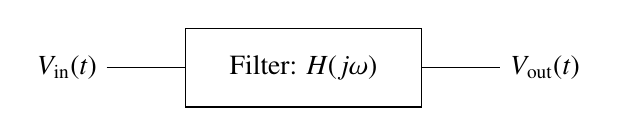
\begin{tikzpicture}
    % Draw the filter rectangle
    \draw (0,0) rectangle (3,1) node[midway] {Filter: $H(j\omega)$};
    
    % Draw the input and output labels
    \draw (-1,0.5) node[left] {$V_{\text{in}}(t)$} -- (0,0.5);
    \draw (3,0.5) -- (4,0.5) node[right] {$V_{\text{out}}(t)$};
\end{tikzpicture}
    \caption{Filter Equivalent of Circuit}
    \label{fig:2_gate.22.ee.31}
\end{figure}
\begin{align}
    H(j\omega) &= \brak{\frac{\sqrt{1 + 100\omega^2 C^2}}{2\sqrt{1 + 121\omega^2 C^2}}}e^{j(\tan^{-1}(10\omega C) - \tan^{-1}(11\omega C))}\\
    &= \brak{\frac{\sqrt{1 + 100\omega^2 C^2}}{2\sqrt{1 + 121\omega^2 C^2}}}e^{j\tan^{-1}\brak{\frac{-\omega C}{1 + 110\omega^2 C^2}}}\\
    \therefore V_{out}(t) &= 10\abs{H(j\omega)}\cos(\omega t + \angle H(j\omega))\\
    &= \frac{5\sqrt{1 + 100\omega^2 C^2}}{\sqrt{1 + 121\omega^2 C^2}}\cos\brak{\omega t -\tan^{-1}\brak{\frac{\omega C}{1 + 110\omega^2 C^2}}}
\end{align}
\begin{figure}[!h]
    \centering
    \includegraphics[width = \columnwidth]{2022/EE/31/figs/V_out_plot.png}
    \caption{Plot of $V_{out}(t)$ at $t=0$ w.r.t $\omega$}
    \label{fig:3_gate.22.ee.31}
\end{figure}

As $\omega \rightarrow 0$, $V_{in}(t)$ approaches being a D.C. input source ($10V$).

$\therefore$ substituting $\omega = 0$, we get:
\begin{align}
    V_{out}(t) &= 5V
\end{align}

%\end{document}


\pagebreak

\item An ideal OPAMP circuit with a sinusoidal input is shown in the figure. The 3dB frequency is the frequency at which the magnitude of the voltage gain decreases by 3 dB from the maximum value. Which of the options is/are correct?

\begin{figure}[H]
  \centering
  \begin{circuitikz}

\ctikzset{bipoles/length=1cm}                           
\draw (0, 0) node[op amp] (opamp) {};
\draw (opamp.-) to[R,l_= $1k\Omega$,-] (-2.5, 0.35) -- (-2.7, 0.35) to[C,l_=$1\mu F$,-](-3.35,0.35)  (-3.25,-0.5) node[ground]{};                                 
\draw (opamp.-) to[short,*-] ++(0,0.5) coordinate (leftC) to[R= $2k\Omega$] (leftC -| opamp.out)to[short,-*] (opamp.out) to [short,-*] (1.5,0) (1.5,-0.5) node[ground]{};
\draw (opamp.+) -- (-1,-0.35) to (-1,-0.5) node[ground]{}
;
\draw[thick] (opamp.up) -- +(0,0.2) node[right] {\scriptsize$+15V$};
\draw[thick] (opamp.down) -- +(0,-0.2) node[right] {\scriptsize$-15V$};

% Double-sided arrows for input and output voltage
%\draw[thick,postaction={decorate,decoration={markings,mark=at position 1.0 with {\arrow{stealth}}}}] (-3.35,-0.5) -- (-3.35,0.30) node[midway,left] {$V_{in}$};
%\draw[postaction={decorate,decoration={markings,mark=at position 1.0 with {\arrow{stealth}}}}] (-3.35,0.30) -- (-3.35,-0.5){};
%\draw[thick,postaction={decorate,decoration={markings,mark=at position 1.0 with {\arrow{stealth}}}}] (1.6,0) -- (1.6,-0.7) node[midway,right] {$V_{out}$};
%\draw[postaction={decorate,decoration={markings,mark=at position 1.0 with {\arrow{stealth}}}}] (1.6,-0.7) -- (1.6,0) {};
 
 
\draw[thick, postaction={decorate,decoration={markings,mark=at position 0 with {\node[left] {\scriptsize$-$}; \draw[-latex](0.2,0)--(0,0);},mark=at position 1 with {\node[left] {\scriptsize$+$}; \draw[-latex] (0,0)--(0.2,0);}}}] (-3.35,-0.7) -- (-3.35,0.1) node[midway,left] {\scriptsize$V_{in}$};
\draw[thick, postaction={decorate,decoration={markings,mark=at position 0 with {\node[right] {\scriptsize$+$}; \draw[-latex] (0.2,0)--(0,0);},mark=at position 1 with {\node[right] {\scriptsize$-$}; \draw[-latex] (0,0)--(0.3,0);}}}] (1.6,0) -- (1.6,-0.5) node[midway,right] {\scriptsize$V_{out}$};
                                                          \end{circuitikz}                                        


  \label{fig:26fig1}
\end{figure}

\begin{enumerate}[label=(\Alph*)]
\item The circuit is a low pass filter.\\
\item The circuit is a high pass filter.\\
\item The 3 dB frequency is 1000rad/s.\\
\item The 3 dB frequency is $\frac{1000}{3}$rad/s.\\
\end{enumerate}
\hfill(GATE EC 2022)\\
\solution
\let\negmedspace\undefined
\let\negthickspace\undefined
\documentclass[journal,12pt,twocolumn]{IEEEtran}
\usepackage{cite}
\usepackage{amsmath,amssymb,amsfonts,amsthm}
\usepackage{algorithmic}
\usepackage{graphicx}
\usepackage{textcomp}
\usepackage{xcolor}
\usepackage{txfonts}
\usepackage{listings}
\usepackage{enumitem}
\usepackage{mathtools}
\usepackage{gensymb}
\usepackage{comment}
\usepackage[breaklinks=true]{hyperref}
\usepackage{tkz-euclide} % loads  TikZ and tkz-base
\usepackage{listings}
\usepackage[latin1]{inputenc}                                
\usepackage{color}                                            
\usepackage{array}                                            
\usepackage{longtable}                                       
\usepackage{calc}                                             
\usepackage{multirow}                                         
\usepackage{hhline}                                           
\usepackage{ifthen}                                           
\usepackage{lscape}
\usepackage{caption}
\usepackage{subcaption}
\usepackage{float}
\usepackage{circuitikz}
\usetikzlibrary{decorations.markings} 


\newtheorem{theorem}{Theorem}[section]
\newtheorem{problem}{Problem}
\newtheorem{proposition}{Proposition}[section]
\newtheorem{lemma}{Lemma}[section]
\newtheorem{corollary}[theorem]{Corollary}
\newtheorem{example}{Example}[section]
\newtheorem{definition}[problem]{Definition}
%\newtheorem{thm}{Theorem}[section] 
%\newtheorem{defn}[thm]{Definition}
%\newtheorem{algorithm}{Algorithm}[section]
%\newtheorem{cor}{Corollary}
\newcommand{\BEQA}{\begin{eqnarray}}
\newcommand{\EEQA}{\end{eqnarray}}
\newcommand{\define}{\stackrel{\triangle}{=}}
\theoremstyle{remark}
\newtheorem{rem}{Remark}
%\bibliographystyle{ieeetr}

\begin{document}

%
\providecommand{\pr}[1]{\ensuremath{\Pr\left(#1\right)}}
\providecommand{\prt}[2]{\ensuremath{p_{#1}^{\left(#2\right)} }}        % own macro for this question
\providecommand{\qfunc}[1]{\ensuremath{Q\left(#1\right)}}
\providecommand{\sbrak}[1]{\ensuremath{{}\left[#1\right]}}
\providecommand{\lsbrak}[1]{\ensuremath{{}\left[#1\right.}}
\providecommand{\rsbrak}[1]{\ensuremath{{}\left.#1\right]}}
\providecommand{\brak}[1]{\ensuremath{\left(#1\right)}}
\providecommand{\lbrak}[1]{\ensuremath{\left(#1\right.}}
\providecommand{\rbrak}[1]{\ensuremath{\left.#1\right)}}
\providecommand{\cbrak}[1]{\ensuremath{\left\{#1\right\}}}
\providecommand{\lcbrak}[1]{\ensuremath{\left\{#1\right.}}
\providecommand{\rcbrak}[1]{\ensuremath{\left.#1\right\}}}
\newcommand{\sgn}{\mathop{\mathrm{sgn}}}
\providecommand{\abs}[1]{\left\vert#1\right\vert}
\providecommand{\res}[1]{\Res\displaylimits_{#1}} 
\providecommand{\norm}[1]{\left\lVert#1\right\rVert}
%\providecommand{\norm}[1]{\lVert#1\rVert}
\providecommand{\mtx}[1]{\mathbf{#1}}
\providecommand{\mean}[1]{E\left[ #1 \right]}
\providecommand{\cond}[2]{#1\middle|#2}
\providecommand{\fourier}{\overset{\mathcal{F}}{ \rightleftharpoons}}
\newenvironment{amatrix}[1]{%
  \left(\begin{array}{@{}*{#1}{c}|c@{}}
}{%
  \end{array}\right)
}
%\providecommand{\hilbert}{\overset{\mathcal{H}}{ \rightleftharpoons}}
%\providecommand{\system}{\overset{\mathcal{H}}{ \longleftrightarrow}}
        %\newcommand{\solution}[2]{\textbf{Solution:}{#1}}
\newcommand{\solution}{\noindent \textbf{Solution: }}
\newcommand{\cosec}{\,\text{cosec}\,}
\providecommand{\dec}[2]{\ensuremath{\overset{#1}{\underset{#2}{\gtrless}}}}
\newcommand{\myvec}[1]{\ensuremath{\begin{pmatrix}#1\end{pmatrix}}}
\newcommand{\mydet}[1]{\ensuremath{\begin{vmatrix}#1\end{vmatrix}}}
\newcommand{\myaugvec}[2]{\ensuremath{\begin{amatrix}{#1}#2\end{amatrix}}}
\providecommand{\rank}{\text{rank}}
\providecommand{\pr}[1]{\ensuremath{\Pr\left(#1\right)}}
\providecommand{\qfunc}[1]{\ensuremath{Q\left(#1\right)}}
        \newcommand*{\permcomb}[4][0mu]{{{}^{#3}\mkern#1#2_{#4}}}
\newcommand*{\perm}[1][-3mu]{\permcomb[#1]{P}}
\newcommand*{\comb}[1][-1mu]{\permcomb[#1]{C}}
\providecommand{\qfunc}[1]{\ensuremath{Q\left(#1\right)}}
\providecommand{\gauss}[2]{\mathcal{N}\ensuremath{\left(#1,#2\right)}}
\providecommand{\diff}[2]{\ensuremath{\frac{d{#1}}{d{#2}}}}
\providecommand{\myceil}[1]{\left \lceil #1 \right \rceil }
\newcommand\figref{Fig.~\ref}
\newcommand\tabref{Table~\ref}
\newcommand{\sinc}{\,\text{sinc}\,}
\newcommand{\rect}{\,\text{rect}\,}
%%
%       %\newcommand{\solution}[2]{\textbf{Solution:}{#1}}
%\newcommand{\solution}{\noindent \textbf{Solution: }}
%\newcommand{\cosec}{\,\text{cosec}\,}
%\numberwithin{equation}{section}
%\numberwithin{equation}{subsection}
%\numberwithin{problem}{section}
%\numberwithin{definition}{section}
%\makeatletter
%\@addtoreset{figure}{problem}
%\makeatother

%\let\StandardTheFigure\thefigure
\let\vec\mathbf

\bibliographystyle{IEEEtran}

\vspace{3cm}
\title{Assignment}
\author{EE23BTECH11001 - Aashna Sahu}
\maketitle
\bigskip

\renewcommand{\thefigure}{\theenumi}
\renewcommand{\thetable}{\theenumi}
%\renewcommand{\theequation}{\theenumi}

Q:An ideal OPAMP circuit with a sinusoidal input is shown in the figure. The 3dB frequency is the frequency at which the magnitude of the voltage gain decreases by 3 dB from the maximum value. Which of the options is/are correct?

\begin{figure}[H]
  \centering
  \begin{circuitikz}

\ctikzset{bipoles/length=1cm}                           
\draw (0, 0) node[op amp] (opamp) {};
\draw (opamp.-) to[R,l_= $1k\Omega$,-] (-2.5, 0.35) -- (-2.7, 0.35) to[C,l_=$1\mu F$,-](-3.35,0.35)  (-3.25,-0.5) node[ground]{};                                 
\draw (opamp.-) to[short,*-] ++(0,0.5) coordinate (leftC) to[R= $2k\Omega$] (leftC -| opamp.out)to[short,-*] (opamp.out) to [short,-*] (1.5,0) (1.5,-0.5) node[ground]{};
\draw (opamp.+) -- (-1,-0.35) to (-1,-0.5) node[ground]{}
;
\draw[thick] (opamp.up) -- +(0,0.2) node[right] {\scriptsize$+15V$};
\draw[thick] (opamp.down) -- +(0,-0.2) node[right] {\scriptsize$-15V$};

% Double-sided arrows for input and output voltage
%\draw[thick,postaction={decorate,decoration={markings,mark=at position 1.0 with {\arrow{stealth}}}}] (-3.35,-0.5) -- (-3.35,0.30) node[midway,left] {$V_{in}$};
%\draw[postaction={decorate,decoration={markings,mark=at position 1.0 with {\arrow{stealth}}}}] (-3.35,0.30) -- (-3.35,-0.5){};
%\draw[thick,postaction={decorate,decoration={markings,mark=at position 1.0 with {\arrow{stealth}}}}] (1.6,0) -- (1.6,-0.7) node[midway,right] {$V_{out}$};
%\draw[postaction={decorate,decoration={markings,mark=at position 1.0 with {\arrow{stealth}}}}] (1.6,-0.7) -- (1.6,0) {};
 
 
\draw[thick, postaction={decorate,decoration={markings,mark=at position 0 with {\node[left] {\scriptsize$-$}; \draw[-latex](0.2,0)--(0,0);},mark=at position 1 with {\node[left] {\scriptsize$+$}; \draw[-latex] (0,0)--(0.2,0);}}}] (-3.35,-0.7) -- (-3.35,0.1) node[midway,left] {\scriptsize$V_{in}$};
\draw[thick, postaction={decorate,decoration={markings,mark=at position 0 with {\node[right] {\scriptsize$+$}; \draw[-latex] (0.2,0)--(0,0);},mark=at position 1 with {\node[right] {\scriptsize$-$}; \draw[-latex] (0,0)--(0.3,0);}}}] (1.6,0) -- (1.6,-0.5) node[midway,right] {\scriptsize$V_{out}$};
                                                          \end{circuitikz}                                        


  \label{fig:fig1}
\end{figure}



\begin{enumerate}[label=(\Alph*)]
\item The circuit is a low pass filter.\\
\item The circuit is a high pass filter.\\
\item The 3 dB frequency is 1000rad/s.\\
\item The 3 dB frequency is $\frac{1000}{3}$rad/s.\\
\end{enumerate}
\hfill(GATE EC 2022)

\solution

\begin{table}[ht]
  \centering
  \begin{table}[!ht] 
\centering
\setlength{\extrarowheight}{8pt}
\begin{tabular}{|l|l|l|}
    \hline
    \textbf{Parameter} & \textbf{Description} & \textbf{Values}\\
    \hline
     m & load of system &  \\
    \hline
     k & stiffness of system &  \\
    \hline
     $\omega_n$ & Natural frequency & $\sqrt{\frac{k}{m}}$ \\
    \hline
    $\zeta$ & Damping ratio & $\frac{c}{2m\omega_n}$ \\
    \hline
     y\brak{t} & Output of system & \\
    \hline
     x\brak{t} & Input to the system & \\
    \hline
     c & Damping coefficient & \\
    \hline
    T\brak{s} & Transfer function of system & $\frac{Y\brak{s}}{R\brak{s}}$\\
    \hline
  \end{tabular}
  \vspace{4mm}
 \caption{Parameter Table}
 \label{tab:table0_ee_22_39}
\end{table}

  \caption{Input Parameters}
  \label{tab:tab1}
\end{table}

\begin{figure}[H]
  \centering
  \input{codes/circuit2.tex}
  \label{fig:fig1}
\end{figure}

\begin{align}
\frac{V_{in}-V}{\frac{1}{sC}+R_1}=\frac{V-V_{out}}{R_2}
\end{align}
As Op-Amp is ideal
\begin{align}
V=V^+=0V\\
\abs{\frac{V_{out}}{V_{in}}}=\frac{sCR_2}{1+sCR_1}\\
H(s)=\frac{sCR_2}{1+sCR_1}
\label{eq:eq4}
\end{align}
Keeping $s=j\omega$\\
For determining nature of Filter\\
Put $j\omega=0$
\begin{align}
H(j\omega)=0
\end{align}
Put $j\omega\rightarrow \infty$
\begin{align}
H(j\omega)=\frac{R_2}{R_1}=2\quad (\text{Finite})
\end{align}\\
$\therefore$ It is high pass filter.\\

On simplifying \eqref{eq:eq4} further
\begin{align}
H(j\omega)=\frac{R_2}{R_1}\left(\frac{j\omega}{j\omega+\frac{1}{CR_1}}\right)\\
\abs{H(j\omega)}_{max}=\frac{R_2}{R_1} \label{eq:eq8}\\
\abs{H(j\omega)}_{\omega=\omega_c}=\frac{R_2}{R_1}\abs{\frac{j\omega_c}{j\omega_c+\frac{1}{CR_1}}}
\label{eq:eq9}
\end{align}
%\textbf{Alternate}\\
%Generally for first order transfer function

%\begin{align}
%H(s)|_{LPF}=\frac{1}{s+\omega}\\
%H(s)|_{HPF}=\frac{s}{s+\omega}
%\label{eq:eq8}
%\end{align}
Given: 
\begin{align}
20\log(\abs{H(j\omega)}_{max})-20\log(\abs{H(j\omega)}_{\omega=\omega_c})=3 dB
\end{align}
\begin{align}
\frac{\abs{H(j\omega)}_{max}}{\abs{H(j\omega)}_{\omega=\omega_c}}=\sqrt 2
\end{align}
 
From \eqref{eq:eq8} and \eqref{eq:eq9}
\begin{align}
\frac{R_2}{R_1}\abs{\frac{j\omega_c}{j\omega_c+\frac{1}{CR_1}}}&=\frac{1}{\sqrt 2}\frac{R_2}{R_1}\\
\abs{\frac{j\omega_c}{j\omega_c+\frac{1}{CR_1}}}&=\frac{1}{\sqrt 2}\\
\implies \omega_c &= \frac{1}{CR_1}
\end{align}
From \tabref{tab:tab1}
\begin{align}
\omega_c= 1000 \text{rad/s}
\end{align}
Where $\omega_c$ is 3 dB frequency.\\

Finally, Correct options are (B) and (C).

\begin{figure}[H]
  \centering
  \includegraphics[width=1.0\columnwidth]{figs/plot1.png}
  \caption{\centering Frequency response plot}
  \label{fig:fig1}
\end{figure}
\end{document}



\pagebreak

\item A series $RLC$ circuit with $R = 10 \Omega$, $L = 50 mH$ and $C = 100 \micro F$ connected to
$200$ $V$, $50$ Hz supply consumes power $P$. The value of $L$ is changed such that this
circuit consumes same power $P$ but operates with lagging power factor. The new
value of L is $\hrulefill$ $mH$ (rounded off to two decimal places).
\hfill(GATE 33 BM 2022)

\solution
\iffalse
\let\negmedspace\undefined
\let\negthickspace\undefined
\documentclass[journal,12pt,twocolumn]{IEEEtran}
\usepackage{cite}
\usepackage{amsmath,amssymb,amsfonts,amsthm}
\usepackage{algorithmic}
\usepackage{graphicx}
\usepackage{textcomp}
\usepackage{xcolor}
\usepackage{txfonts}
\usepackage{listings}
\usepackage{enumitem}
\usepackage{mathtools}
\usepackage{gensymb}
\usepackage{comment}
\usepackage[breaklinks=true]{hyperref}
\usepackage{tkz-euclide} 
\usepackage{tikz}
\usepackage{circuitikz}
\usepackage{listings}
\usepackage{gvv}                                        
\def\inputGnumericTable{}                                 
\usepackage[latin1]{inputenc}                                
\usepackage{color}                                            
\usepackage{array}                                            
\usepackage{longtable}                                       
\usepackage{calc}                                             
\usepackage{multirow}                                         
\usepackage{hhline}                                           
\usepackage{ifthen}                                           
\usepackage{lscape}
\usepackage{caption}
\newtheorem{theorem}{Theorem}[section]
\newtheorem{problem}{Problem}
\newtheorem{proposition}{Proposition}[section]
\newtheorem{lemma}{Lemma}[section]
\newtheorem{corollary}[theorem]{Corollary}
\newtheorem{example}{Example}[section]
\newtheorem{definition}[problem]{Definition}
\newcommand{\BEQA}{\begin{eqnarray}}
\newcommand{\EEQA}{\end{eqnarray}}
\newcommand{\define}{\stackrel{\triangle}{=}}
\theoremstyle{remark}
\newtheorem{rem}{Remark}
\begin{document}
\parindent 0px
\bibliographystyle{IEEEtran}
\vspace{3cm}

\title{GATE 2022 33.BM}
\author{EE23BTECH11012 - Chavan Dinesh$^{*}$% <-this % stops a space
}
\maketitle
\newpage
\bigskip

\renewcommand{\thefigure}{\arabic{figure}}
\renewcommand{\thetable}{\arabic{table}}
\large\textbf{\textsl{Question:}}
A series $RLC$ circuit with $R = 10 \Omega$, $L = 50 mH$ and $C = 100 \micro F$ connected to
$200$ $V$, $50$ Hz supply consumes power $P$. The value of $L$ is changed such that this
circuit consumes same power $P$ but operates with lagging power factor. The new
value of L is $\hrulefill$ $mH$ (rounded off to two decimal places).
\hfill(GATE 33 BM 2022)

\solution
\fi
\begin{table}[htbp]
    \centering
    \begin{tabular}{|c|c|c|}
\hline
   \textbf{Parameter}  & \textbf{Description} & \textbf{Value}\\
   \hline
   $R$   & Resistance & $10 \Omega$\\
   \hline
  $C$ & Capacitance & $100 \micro F$ \\
  \hline
  $L_{old}$ & Inductor & $50mH$\\
  \hline
  $L_{new}$ & New Inductor &    \\
  \hline
  $Z_{old}$ & Old Impedance & \\
  \hline
  $Z^*$ &New Impedance & \\
  \hline
  
\end{tabular}

    \caption{}
    \label{tab:input_parameters.33.BM.2022}
\end{table}

\begin{figure}[!ht]
    \centering
    \documentclass[tikz, border=2mm]{standalone}
\usetikzlibrary{shapes, arrows.meta}

\begin{document}

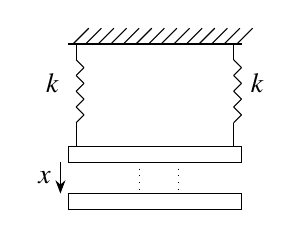
\begin{tikzpicture}
    % Support rod (horizontal)
    \draw (0.4,2) -- (2.6,2); % Shortened the support system
    
    % First Rectangle
    \draw (0.4,0.5) rectangle (2.6,0.7); % Centered the first rectangle
    
    % First Spring (tight rod)
\draw (0.5,1.8) -- (0.5,2);
    \draw (0.5,1.8) -- (0.6,1.7);
    \draw (0.6,1.7) -- (0.5,1.6);
    \draw (0.5,1.6) -- (0.6,1.5);
    \draw (0.6,1.5) -- (0.5,1.4);
    \draw (0.5,1.4) -- (0.6,1.3);
    \draw (.6,1.3) -- (0.5,1.2);
    \draw (0.5,1.2) -- (.6,1.1);
    \draw (.6,1.1) -- (0.5,1);
    \draw (0.5,1)--(0.5,0.7);
    \node at (0.2, 1.5) {$k$};
    
    % Second Rectangle (dotted)
    \draw (0.4,0.1) rectangle (2.6,-0.1);
    
    % Second Spring (tight rod)
    \draw (2.5,1.8) -- (2.5,2);
    \draw (2.5,1.8) -- (2.6,1.7);
    \draw (2.6,1.7) -- (2.5,1.6);
    \draw (2.5,1.6) -- (2.6,1.5);
    \draw (2.6,1.5) -- (2.5,1.4);
    \draw (2.5,1.4) -- (2.6,1.3);
    \draw (2.6,1.3) -- (2.5,1.2);
    \draw (02.5,1.2) -- (2.6,1.1);
    \draw (2.6,1.1) -- (02.5,1);
    \draw (02.5,1)--(02.5,0.7);
    \node at (2.8, 1.5) {$k$};
    
    \foreach \i in {1,...,14}
        \draw ({0.3 + 0.16*\i},2) -- ({0.5 + 0.16*\i},2.2);
    
    \draw[thin, dotted] (1.3,0.5) -- (1.3,0.1);
    \draw[thin, dotted] (1.8,0.5) -- (1.8,0.1);
    
    % Arrow downwards for \delta x
    \draw[->, >=Stealth] (0.3, 0.5) -- node[midway, left] {\(x\)} (0.3, 0.1);
\end{tikzpicture}

\end{document}


    \caption{}
    \label{fig:fig1.33.BM.2022}
\end{figure}

From \figref{fig:fig1.33.BM.2022}

In $s$ - domain,
\begin{figure}[htbp]
    \centering
    \begin{tikzpicture}
\begin{axis}[
    axis lines=middle,
    xmin=-30,
    xmax=30,
    ymin=-0.5,
    ymax=1.5,
    xlabel={$f$},
    ylabel={$H_2(f)$},
    xtick={-15,15},
    ytick={0,1},
    ]
    \addplot [blue, thick] coordinates {(-25,0)(-15,0) (-15,1) (15,1) (15,0)(25,0)};
\end{axis}
\end{tikzpicture}   \label{kk:gateee47Q.2}

\end{figure}

  \begin{align}
      Z = R + sL_{old} + \frac{1}{sC}
  \end{align}
As the circuit consumes same power $P$ but operates with lagging power factor : 

The new impedance($Z^*$) will be :
\begin{align}
    Z^* =  R + sL_{new} + \frac{1}{sC}
\end{align}
Comparing the imaginary parts of the impedances:
\begin{align}
    sL_{old} + \frac{1}{sC} = -\left( sL_{new} + \frac{1}{sC}\right)
    \end{align}
Taking $s = j2\pi f$ :
\begin{align}
     j\left(2\pi fL_{old} - \frac{1}{2\pi fC}\right)  =  -j\left(2\pi fL_{new} - \frac{1}{2\pi fC}\right)
\end{align}
From \tabref{tab:input_parameters.33.BM.2022}:
\begin{align}
    L_{new} \approx 152.7 \text{mH}
\end{align}

% \begin{figure}[ht]
%     \centering
%     \includegraphics[width = \columnwidth]{figs/x_n_stem_plot.png}
%     \caption{}
%     \label{fig:graph1.11.9.3.28}
% \end{figure}



\pagebreak

\item A single-phase full-bridge diode rectifier feeds a resistive load of $50 \Omega$ from a 200 V,
50 Hz single phase AC supply. If the diodes are ideal, then the active power, in watts,
drawn by the load is \rule{1cm}{0.5mm} (round off to nearest integer).  \\
\hfill (GATE EE 32)\\
\solution
\iffalse
\documentclass[journal,12pt,twocolumn]{IEEEtran}
\usepackage{amsmath,amssymb,amsfonts,amsthm}
\usepackage{txfonts}
\usepackage{tkz-euclide}
\usepackage{listings}
\usepackage{gvv}
\usepackage[latin1]{inputenc}
\usepackage{adjustbox}
\usepackage{array}
\usepackage{tabularx}
\usepackage{pgf}
\usepackage{lmodern}
\usepackage{circuitikz}
\usepackage{tikz}
\usepackage{graphicx}
\usepackage[english]{babel}

\begin{document}
\bibliographystyle{IEEEtran}

\vspace{3cm}

\title{}
\author{EE23BTECH11047 - Deepakreddy P
}
\maketitle
\newpage
\bigskip

\noindent \textbf{32} \quad A single-phase full-bridge diode rectifier feeds a resistive load of $50 \Omega$ from a 200 V,
50 Hz single phase AC supply. If the diodes are ideal, then the active power, in watts,
drawn by the load is \rule{1cm}{0.5mm} (round off to nearest integer).  \\
\hfill (GATE EE 32)\\
\solution\\
\fi

\begin{figure}[ht]
  \centering
      \begin{circuitikz}[american]
   \draw (0,8) to [sV=200V](0,-1) to [short](6,-1) to [short](6,0) to [D,l=$D_3$](9,3);
   \draw (0,8) to [short](6,8) to [short](6,6);
   \draw (6,6) to [D,l=$D_1$](9,3);
   \draw (3,3) to [D,l=$D_4$](6,6);
   \draw (3,3) to [D,l=$D_2$](6,0);
   \draw (3,3) to [short](2.5,3) to [crossing, bipoles/crossing/size=1](2.5,-4.8) to [short](12,-4.8) to [R=50$\Omega$](12,3) to [short](9,3);
   \draw (9,3) to [short,i=\Large{I}](12,3);
\end{circuitikz}

  \caption{Circuit-1}
\end{figure}

\begin{figure}[ht]
   \centering
   \includegraphics[width=1.2\columnwidth]{2022/EE/32/figs/gt1.png}
   \caption{Output voltage waveform of single-phase full
bridge rectifier}
\end{figure}


\begin{center}
    \begin{table}[ht]
        \setlength{\arrayrulewidth}{0.3mm}
\setlength{\tabcolsep}{12pt}
\renewcommand{\arraystretch}{1.3}


\begin{center}
\caption{Input Parameters}
\begin{tabular}{ |p{1.7cm}|p{1.7cm}|p{1.7cm}|  }

\hline
 {Symbol}&{Description} & {value}\\
\hline
R & Load Resistance & 50$\Omega$\\
\hline
$V_{rms}$ & RMS Voltage  & 200V\\
\hline
f & Frequency & 50Hz \\
\hline

\end{tabular}
\end{center}

    \end{table}
\end{center}

\begin{align}
    V_{rms} &= 200\\
    P &= \frac{\brak{V_{rms}}^2}{R}\\
    P &= \frac{\brak{200}^2}{50}W\\
    P &= 800W
\end{align}


%\end{document}


\pagebreak

\item The circuit shown is driven by a sinusoidal input voltage, $V_{\text{in}}$, resulting in the output voltage $V_{\text{out}}$. The frequency (in kilohertz) at which the voltage gain is 0 dB is (rounded off to two decimal places).
\begin{figure}[htb]
  \centering
  \documentclass[tikz, border=2mm]{standalone}
\usetikzlibrary{shapes, arrows.meta}

\begin{document}

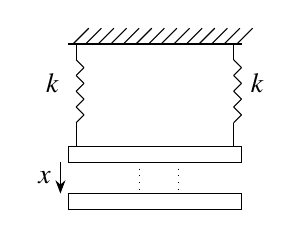
\begin{tikzpicture}
    % Support rod (horizontal)
    \draw (0.4,2) -- (2.6,2); % Shortened the support system
    
    % First Rectangle
    \draw (0.4,0.5) rectangle (2.6,0.7); % Centered the first rectangle
    
    % First Spring (tight rod)
\draw (0.5,1.8) -- (0.5,2);
    \draw (0.5,1.8) -- (0.6,1.7);
    \draw (0.6,1.7) -- (0.5,1.6);
    \draw (0.5,1.6) -- (0.6,1.5);
    \draw (0.6,1.5) -- (0.5,1.4);
    \draw (0.5,1.4) -- (0.6,1.3);
    \draw (.6,1.3) -- (0.5,1.2);
    \draw (0.5,1.2) -- (.6,1.1);
    \draw (.6,1.1) -- (0.5,1);
    \draw (0.5,1)--(0.5,0.7);
    \node at (0.2, 1.5) {$k$};
    
    % Second Rectangle (dotted)
    \draw (0.4,0.1) rectangle (2.6,-0.1);
    
    % Second Spring (tight rod)
    \draw (2.5,1.8) -- (2.5,2);
    \draw (2.5,1.8) -- (2.6,1.7);
    \draw (2.6,1.7) -- (2.5,1.6);
    \draw (2.5,1.6) -- (2.6,1.5);
    \draw (2.6,1.5) -- (2.5,1.4);
    \draw (2.5,1.4) -- (2.6,1.3);
    \draw (2.6,1.3) -- (2.5,1.2);
    \draw (02.5,1.2) -- (2.6,1.1);
    \draw (2.6,1.1) -- (02.5,1);
    \draw (02.5,1)--(02.5,0.7);
    \node at (2.8, 1.5) {$k$};
    
    \foreach \i in {1,...,14}
        \draw ({0.3 + 0.16*\i},2) -- ({0.5 + 0.16*\i},2.2);
    
    \draw[thin, dotted] (1.3,0.5) -- (1.3,0.1);
    \draw[thin, dotted] (1.8,0.5) -- (1.8,0.1);
    
    % Arrow downwards for \delta x
    \draw[->, >=Stealth] (0.3, 0.5) -- node[midway, left] {\(x\)} (0.3, 0.1);
\end{tikzpicture}

\end{document}


\end{figure}
\hfill(GATE IN 2022)\\
\solution
\iffalse
\documentclass[journal,12pt,twocolumn]{IEEEtran}
\usepackage{cite}
\usepackage{amsmath,amssymb,amsfonts,amsthm}
\usepackage{algorithmic}
\usepackage{graphicx}
\usepackage{textcomp}
\usepackage{xcolor}
\usepackage{listings}
\usepackage{enumitem}
\usepackage{mathtools}
\usepackage{gensymb}
\usepackage{comment}
\usepackage[breaklinks=true]{hyperref}
\usepackage{tkz-euclide}
\usepackage{gvv} 
\def\inputGnumericTable{} 
\usepackage[latin1]{inputenc} 
\usepackage{color} 

\newtheorem{theorem}{Theorem}[section]
\newtheorem{problem}{Problem}
\newtheorem{proposition}{Proposition}[section]
\newtheorem{lemma}{Lemma}[section]
\newtheorem{corollary}[theorem]{Corollary}
\newtheorem{example}{Example}[section]
\newtheorem{definition}[problem]{Definition}
\newcommand{\BEQA}{\begin{eqnarray}}
\newcommand{\EEQA}{\end{eqnarray}}
\newcommand{\define}{\stackrel{\triangle}{=}}
\theoremstyle{remark}
\newtheorem{rem}{Remark}

\begin{document}

\bibliographystyle{IEEEtran}
\vspace{3cm}

\title{GATE 2022-IN}
\author{EE23BTECH1205 - Avani Chouhan$^{*}$}
\maketitle
\newpage
\bigskip

\renewcommand{\thefigure}{\theenumi}
\renewcommand{\thetable}{\theenumi}

\vspace{3cm}
\textbf{Question : 18} \\
A signal \( x(t) \) is band-limited between 100 Hz and 200 Hz. A signal \( y(t) \) is related to \( x(t) \) as follows:\\

\( y(t) = x(2t - 5) \)\\
The statement that is always true is \\

\begin{enumerate}
  \item[(A)] \( y(t) \) is band-limited between 50 Hz and 100 Hz
  \item[(B)] \( y(t) \) is band-limited between 100 Hz and 200 Hz
  \item[(C)] \( y(t) \) is band-limited between 200 Hz and 400 Hz
  \item[(D)] \( y(t) \) is not band-limited 
\end{enumerate}

\hfill{(GATE IN 2022)}\\
\textbf{Solution:} \\
\fi
\begin{align}
x(t) &\rightleftharpoons X(\omega) \label{eq1}\\
x(at) &\rightleftharpoons \frac{1}{|a|} X\left(\frac{\omega}{a}\right) \label{eq2}\\
x(2t) &\rightleftharpoons \frac{1}{2} X\left(\frac{\omega}{2}\right) \label{eq3}\\
x(t - t_0) &\rightleftharpoons e^{-j\omega t_0}X(\omega) \label{eq4}\\
x(2t - 5) &\rightleftharpoons e^{-j5\omega} \cdot \frac{1}{2} X\left(\frac{\omega}{2}\right) \label{eq5}
\end{align}

The operation \(x(2t-5)\) compresses time by a factor of 2 and shifts 5 units rightward. This expands the frequency domain, doubling the bandwidth of \(x(t)\) from 100 Hz to 200 Hz to \(y(t)\) between 200 Hz and 400 Hz.\\

Hence, the correct answer is option (C).

%\end{document}


\pagebreak

\item An inductor having a $Q$-factor of 60 is connected in series with a capacitor having a $Q$-factor of 240. The overall $Q$-factor of the circuit is \_\_\_\_\_\_\_\_\_\_. (Round off to the nearest integer) \\
\hfill Gate 2022 EE Question 27\\
\solution
\iffalse
\let\negmedspace\undefined
\let\negthickspace\undefined
\documentclass[journal,12pt,twocolumn]{IEEEtran}
\usepackage{cite}
\usepackage{amsmath,amssymb,amsfonts,amsthm}
\usepackage{algorithmic}
\usepackage{graphicx}
\usepackage{textcomp}
\usepackage{xcolor}
\usepackage{txfonts}
\usepackage{listings}
\usepackage{enumitem}
\usepackage{mathtools}
\usepackage{gensymb}
\usepackage{comment}
\usepackage[breaklinks=true]{hyperref}
\usepackage{tkz-euclide} 
\usepackage{listings}                                   
\def\inputGnumericTable{}                                 
\usepackage[latin1]{inputenc}                                
\usepackage{color}                                            
\usepackage{array}                                            
\usepackage{longtable}                                       
\usepackage{calc}  
\usepackage{circuitikz}                                           
\usepackage{multirow}                                         
\usepackage{hhline}                                           
\usepackage{ifthen}                                           
\usepackage{lscape}
\newtheorem{theorem}{Theorem}[section]
\newtheorem{problem}{Problem}
\newtheorem{proposition}{Proposition}[section]
\newtheorem{lemma}{Lemma}[section]
\newtheorem{corollary}[theorem]{Corollary}
\newtheorem{example}{Example}[section]
\newtheorem{definition}[problem]{Definition}
\newcommand{\BEQA}{\begin{eqnarray}}
\newcommand{\EEQA}{\end{eqnarray}}
\newcommand{\define}{\stackrel{\triangle}{=}}
\newcommand{\brak}[1]{\langle #1 \rangle}
\theoremstyle{remark}
\newtheorem{rem}{Remark}

\begin{document}
\bibliographystyle{IEEEtran}
\vspace{3cm}
\title{\textbf{GATE 2022 EE}}
\author{EE23BTECH11023-ABHIGNYA GOGULA}
\maketitle
\newpage
\bigskip
\renewcommand{\thefigure}{\theenumi}
\renewcommand{\thetable}{\theenumi}
\textbf{Question27:}
\\An inductor having a $Q$-factor of 60 is connected in series with a capacitor having a $Q$-factor of 240. The overall $Q$-factor of the circuit is \_\_\_\_\_\_\_\_\_\_. (Round off to the nearest integer) \\
\hfill Gate 2022 EE Question 27\\
\section*{Solution}
\fi
\begin{circuitikz}
    \draw (0,0) to[R, l=$R_1$] (2,0) to[L, l=$L$] (4,0);
\end{circuitikz}
\begin{align}
Q_1=\frac{\omega_0 L}{R_1}
\end{align}
\begin{circuitikz}
    \draw (0,0) to[R, l=$R_2$] (2,0) to[C, l=$C$] (4,0);
\end{circuitikz}
\begin{align}
Q_2=\frac{1}{\omega_0 C R_2}
\end{align}
at resonance as $\omega_0 L =\frac{1}{\omega_0 C}$ hence
\begin{align}
Q_2=\frac{\omega_0 L}{R_2}
\end{align}
\begin{circuitikz}
    \draw (0,0) to[R, l=$R_1$] (2,0) to[L, l=$L$] (4,0) to[R, l=$R_2$] (6,0) to[C, l=$C$] (8,0);
\end{circuitikz}
\begin{align}
Q = \frac{\omega_0 L}{R_1+R_2}\\
Q = \frac{1}{\frac{R_1}{\omega_0 L}+\frac{R_2}{\omega_0 L}}
\end{align}
\begin{equation}
Q =\frac{Q_1 Q_2}{Q_1+Q_2}
\label{eq:EE 27eq1}
\end{equation}
then from \eqref{eq:EE 27eq1}
\begin{align}
Q=\frac{60 \times 240}{60+240}\\
Q=48
\end{align}
%\end{document}

\pagebreak

\item In the circuit shown, the switch is initially closed. It is opened at t= 0 s and
remains open thereafter. The time (in milliseconds) at which the output voltage
$V_{out}$ becomes LOW is  (round off to three decimal places)\hfill(GATE IN 2022)\\
\begin{figure}[ht]
\centering
\begin{circuitikz}

    % Draw resistors and voltage source
    \draw (0,0) to[resistor={{$600\Omega$}}] (2,0) ;
    \draw (2,0) -- (2,-1) to[resistor={{$400\Omega$}}] (0,-1) node[ground]{};
    \draw (2,-0.5) --(3,-0.5) -- (3,-2.5);
    
    \draw (5,-3) node[op amp] (opamp) {};
    \draw (opamp.up) ++(0,0.3) node[above] {$+5V$};
     \draw (opamp.down) ++(0,-0.3) node[below] {$-5V$};
     \draw (5,-2.5) -- (5,-2.1);
    \draw (opamp.-) -- (3,-2.5);
    \draw (5,-3.5) -- (5,-3.9);
    \draw (opamp.out) -- (6,-3) node[right] {$V_{out}$};
    \draw (opamp.+) -- (3,-3.5) -- (3,-4.5);
    \draw (3,-4.5) to[resistor={{$5k\Omega$}}] (3,-6.5)node[ground]{};
    \draw (3,-4.5) -- (0.8,-4.5);
    \draw (0.8,-4.5) to[C, l=$0.1\mu F$] (0.8,-6.5)node[ground]{};
    \draw (0,0) -- (-1.5,0)node[above] {$+5V$};
    \draw (-1.5,0) -- (-1.5,-1) to [resistor={{$1k\Omega$}}] (-1.5,-3);
    \draw (-1.5,-3) to[ospst, l={$t= 0s$}] (-1.5,-4.5);
    \draw (-1.5,-4.5) -- (0.8,-4.5);    
\end{circuitikz}
\end{figure}

\solution\\
\iffalse
\documentclass[journal,12pt,twocolumn]{IEEEtran}
\usepackage{amsmath,amssymb,amsfonts,amsthm}
\usepackage{txfonts}
\usepackage{tkz-euclide}
\usepackage{listings}
\usepackage{gvv}
\usepackage[latin1]{inputenc}
\usepackage{array}
\usepackage{pgf}
\usepackage{lmodern}
\usepackage{amsmath}
\usepackage{circuitikz}
\begin{document}
\bibliographystyle{IEEEtran}

\title{GATE 2022[IN]-64}
\author{EE23BTECH11066 - Yakkala Amarnath Karthik}
\maketitle
\bibliographystyle{IEEEtran}

\textbf{Question:}\\ \\
In the circuit shown, the switch is initially closed. It is opened at t= 0 s and
remains open thereafter. The time (in milliseconds) at which the output voltage
$V_{out}$ becomes LOW is  (round off to three decimal places)\hfill(GATE IN 2022)\\
\begin{figure}[ht]
\centering
\begin{circuitikz}

    % Draw resistors and voltage source
    \draw (0,0) to[resistor={{$600\Omega$}}] (2,0) ;
    \draw (2,0) -- (2,-1) to[resistor={{$400\Omega$}}] (0,-1) node[ground]{};
    \draw (2,-0.5) --(3,-0.5) -- (3,-2.5);
    
    \draw (5,-3) node[op amp] (opamp) {};
    \draw (opamp.up) ++(0,0.3) node[above] {$+5V$};
     \draw (opamp.down) ++(0,-0.3) node[below] {$-5V$};
     \draw (5,-2.5) -- (5,-2.1);
    \draw (opamp.-) -- (3,-2.5);
    \draw (5,-3.5) -- (5,-3.9);
    \draw (opamp.out) -- (6,-3) node[right] {$V_{out}$};
    \draw (opamp.+) -- (3,-3.5) -- (3,-4.5);
    \draw (3,-4.5) to[resistor={{$5k\Omega$}}] (3,-6.5)node[ground]{};
    \draw (3,-4.5) -- (0.8,-4.5);
    \draw (0.8,-4.5) to[C, l=$0.1\mu F$] (0.8,-6.5)node[ground]{};
    \draw (0,0) -- (-1.5,0)node[above] {$+5V$};
    \draw (-1.5,0) -- (-1.5,-1) to [resistor={{$1k\Omega$}}] (-1.5,-3);
    \draw (-1.5,-3) to[ospst, l={$t= 0s$}] (-1.5,-4.5);
    \draw (-1.5,-4.5) -- (0.8,-4.5);    
\end{circuitikz}
\end{figure}
 

\textbf{Solution:}\\ 
\fi
At t$=0^-$, when the switch is closed,\\
The voltage across the capacitor is:
\begin{align}
V_c\brak{0^-}&=5\times\frac{5}{5+1}\\
&=\frac{25}{6}V
\end{align}
$V_c\brak{0^-}$ is also the non inverting voltage of the OP-AMP\\ \\
At $t=0^+$, when the switch is open,\\
The voltage across inverting terminal is:
\begin{align}
V_I&=5\times\frac{600}{600+400}\\
&=2V
\end{align}
Analysing the circuit at t=$0^+$ in laplace domain:\\ 
\begin{figure}
\centering
\begin{circuitikz}[american]

    % Draw resistors and voltage source
    \draw (0,0) node[left] {$5V$}to[resistor={{$600\Omega$}}] (2,0) ;
    \draw (2,0) -- (2,-1) to[resistor={{$400\Omega$}}] (0,-1) node[ground]{};
    \draw (2,-0.5) --(3,-0.5) -- (3,-2.5);
    
    \draw (5,-3) node[op amp] (opamp) {};
    \draw (opamp.up) ++(0,0.3) node[above] {$+5V$};
    \draw (5,-2.5) -- (5,-2.1);
     \draw (opamp.down) ++(0,-0.3) node[below] {$-5V$};
      \draw (5,-3.5) -- (5,-3.9);
    \draw (opamp.-) -- (3,-2.5)node[left]{$V_I=2V$};
    \draw (opamp.out) -- (6,-3) --(7,-3) node[right] {$V_{out}$};
    \draw (opamp.+) -- (3,-3.5)node[above]{$V_{NI}$} -- (3,-4.5);
    \draw (3,-4.5) to[resistor={{$5k\Omega$}}] (3,-7.5)node[ground]{};
  % \draw (3,-4.5) -- (0.8,-4.5);
    \draw (3,-4.5) to [V, v=$\frac{25}{6s}V$] (0.8,-4.5);
    \draw (0.8,-4.5) to[resistor={{$\frac{1}{10^{-7}s}\Omega$}}] (0.8,-7.5)node[ground]{};
\end{circuitikz}
    \caption{circuit diagram in laplace domain at $t=0^+$}
\end{figure}


Using voltage divider rule,
\begin{align}
V_{NI}\brak{s}&=V\times\sbrak{\frac{R}{R+\frac{1}{sC}}}\\
    &=\frac{25}{6s}\times\sbrak{\frac{s}{s+\frac{1}{RC}}}\\
    &=\frac{25}{6}\times\sbrak{\frac{1}{s+\frac{1}{RC}}}
\end{align}
Applying inverse laplace:
\begin{align}
    V_{NI}\brak{t}&=\frac{25}{6} e^{\frac{-t}{RC}}\\
    \implies  2&=\frac{25}{6}\times e^{\frac{-t}{RC}}\\
  \implies  t&=RC\ln\brak{\frac{25}{12}}\\
    &=0.1\times10^{-6}\times5\times10^{3}\ln{\brak{\frac{25}{12}}}\\
    &=0.367ms
\end{align}
%\end{document}

\pagebreak

\item The steady state output $v_{out}$ of the circuit shown below, will
\begin{figure}[h]
    \centering
    \begin{circuitikz}[american voltages]
    \draw (0,0) node[op amp] (opamp) {};
    \draw (opamp.+) node[above]{$v_{+}$} to (-2,-0.5);
    \draw (opamp.-) node[above]{$v_{-}$} to (-2, 0.5);
    \draw (opamp.out) to (2, 0)node[right]{$v_{out}$};
    \draw (opamp.down) to (-0.1, -1) node[below]{$-v_{EE}$};
    \draw (opamp.up) to (-0.1, 1)node[above]{$+v_{DD}$};
    \draw (-2,0.5) to [R, l_=$R_1$](-3,0.5) to (-3.5, 0.5) to [V, l_=$0.1v$] (-3.5, -2) node[ground]{};
    \draw (-2, -0.5) to [R, l=$R_2$] (-2, -2) node[ground]{};
    \draw (-1.5,0.5) to (-1.5, 2) to [C, l=$C_1$] (1.5, 2) to (1.5, 0);
\end{circuitikz}

    \caption{Circuit}
    \label{fig: 217.EE.16.1}
\end{figure}

\begin{enumerate}
    \item saturate to $+V_{DD}$
    \item saturate to $-V_{EE}$
    \item become equal to $0.1V$
    \item become equal to $-0.1V$
\end{enumerate}
\solution
\iffalse
\documentclass[journal,12pt,twocolumn]{IEEEtran}
\usepackage{amsmath,amssymb,amsfonts,amsthm}
\usepackage{txfonts}
\usepackage{tkz-euclide} 
\usepackage{listings}
\usepackage{gvv}       
\usepackage[latin1]{inputenc}   
\usepackage{array}  
\usepackage{tikz}
\usepackage{circuitikz}

\begin{document}

\bibliographystyle{IEEEtran}

\vspace{3cm}

\title{}
\author{EE23BTECH11217 - Prajwal M$^{*}$
}
\maketitle
\newpage
\bigskip

\renewcommand{\thefigure}{\theenumi}
\renewcommand{\thetable}{\theenumi}

\section*{EE 16}
The steady state output $V_{out}$ of the circuit shown below, will
\begin{figure}[h]
    \centering
    \begin{circuitikz}[american voltages]
    \draw (0,0) node[op amp] (opamp) {};
    \draw (opamp.+) node[above]{$v_{+}$} to (-2,-0.5);
    \draw (opamp.-) node[above]{$v_{-}$} to (-2, 0.5);
    \draw (opamp.out) to (2, 0)node[right]{$v_{out}$};
    \draw (opamp.down) to (-0.1, -1) node[below]{$-v_{EE}$};
    \draw (opamp.up) to (-0.1, 1)node[above]{$+v_{DD}$};
    \draw (-2,0.5) to [R, l_=$R_1$](-3,0.5) to (-3.5, 0.5) to [V, l_=$0.1v$] (-3.5, -2) node[ground]{};
    \draw (-2, -0.5) to [R, l=$R_2$] (-2, -2) node[ground]{};
    \draw (-1.5,0.5) to (-1.5, 2) to [C, l=$C_1$] (1.5, 2) to (1.5, 0);
\end{circuitikz}

    \caption{circuit}
    \label{fig: 217.EE.16.1}
\end{figure}

\begin{enumerate}
    \item saturate to $+V_{DD}$
    \item saturate to $-V_{EE}$
    \item become equal to $0.1V$
    \item become equal to $-0.1V$
\end{enumerate}

\noindent Solution: \\

\fi
\begin{table}[h]
    \centering
    \begin{tabular}{|c|c|}
\hline
    Parameters & Description \\\hline
    $v_{\text{out}}$  & Steady State Output Voltage  \\\hline
    $V_{\text{out}}$ & Laplace Transform of $v_{\text{out}}$\\\hline
\end{tabular}

    \caption{Parameter description}
\label{tab: 217.EE.16.1}
\end{table}

\begin{figure}[h]
    \centering
    \begin{circuitikz}[american voltages]
    \draw (0,0) node[op amp] (opamp) {};
    \draw (opamp.+) node[above]{$V_{+}$} to (-2,-0.5);
    \draw (opamp.-) node[above]{$V_{-}$}to (-2, 0.5);
    \draw (opamp.out) to (2, 0)node[right]{$V_{out}$};
    \draw (opamp.down) to (-0.1, -1) node[below]{$-V_{EE}$};
    \draw (opamp.up) to (-0.1, 1)node[above]{$+V_{DD}$};
    \draw (-2,0.5) to [R, l_=$R_1$](-3,0.5) to (-3.5, 0.5) to [V, l_=$0.1V$] (-3.5, -2) node[ground]{};
    \draw (-2, -0.5) to [R, l=$R_2$] (-2, -2) node[ground]{};
    \draw (-1.5,0.5) to (-1.5, 2) to [R, l=$\frac{1}{sC_1}$] (1.5, 2) to (1.5, 0);
\end{circuitikz}

    \caption{s-domain circuit}
    \label{fig: 217.EE.16.2}
\end{figure}

for an ideal OP amp,
\begin{align}
    V_+ & = 0V \\
    V_- & = 0V\label{217.EE.16.1}
\end{align}
using KVL,
\begin{align}
    0 & = \frac{V_{-} - 0.1}{R_1} + C_1 s\brak{V_{-} - V_{out}}\\
    V_{out} & = \frac{V_- -0.1}{R_1C_1s} + V_-\\
    & = -\frac{0.1}{R_1C_1s} & \text{using \eqref{217.EE.16.1}}\\
    V_{out} & \system{L^-} v_{out}\\
    v_{out} & = -\frac{0.1}{R_1C_1}t\\
    v_{out} & = max\cbrak{-v_{EE}, -\frac{1}{R_1C_1}t}
\end{align}

Hence, $v_{out}$ saturates to $-v_{EE}$

\pagebreak

\item For the circuit shown below with ideal diodes, the output will be :\\
\brak{A} $V_{\text{out}} = V_{\text{in}} \text{ for } V_{\text{in}}>0 $ \\
\brak{B} $V_{\text{out}} = V_{\text{in}} \text{ for } V_{\text{in}}<0 $ \\
\brak{C} $V_{\text{out}} = -V_{\text{in}} \text{ for } V_{\text{in}}>0 $ \\
\brak{D} $V_{\text{out}} = -V_{\text{in}} \text{ for } V_{\text{in}}<0 $ \\

\begin{figure}[ht]
  \centering
  \resizebox{0.55\columnwidth}{!}{\input{2022/EE/25/figs/figure.tex}}
  \caption{Gate EE 25 fig-1}
  \label{fig:gate_ee_25_1}
\end{figure}
\solution
\input{2022/EE/25/gate_ee_25.tex}
\pagebreak

\item Consider an FM broadcast that employs the pre-emphasis filter with frequency response \\
    \begin{align*}
        H_{pe}\brak{\omega}= 1+ \frac{j\omega}{\omega _0},
    \end{align*}
    where $\omega_0=10^4$ rad/sec. \\
    For the network shown in the figure to act as a corresponding de-emphasis filter, the
appropriate pair(s) of (R,C) values is/are 
\underline{\hspace{1in}}
\begin{figure}[htb]
  \centering
  \begin{center}
    \begin{circuitikz}
		\draw
		(0,0)  to[resistor,*-,l=$R$] (4,0)
		to[capacitor,l=$C$] (4,-4) to (7,-4)
		(4,0) -- (7,0)
		(4,-4) to[short,-*] (0,-4);
		\node[below left] at (0,0){$+$};
		\node[above left] at (0,-4){$-$};
		\node[below right] at (7,0){$+$};
		\node[above right] at (7,-4){$-$};
		\draw [<->] (0,-0.3) -- (0,-3.7);
		\node[left] at (0,-2){input};
		\draw [<->] (7,-0.3) -- (7,-3.7);
		\node[right] at (7,-2){output};
	\end{circuitikz}
\end{center}
\end{figure}
\hfill(GATE EC 51)\\
\begin{enumerate}
    \item[A.] $R=1k\ohm$, $C=0.1\micro F$
    \item[B.] $R=2k\ohm$, $C=1\micro F$
    \item[C.] $R=1k\ohm$, $C=2\micro F$
    \item[D.] $R=2k\ohm$, $C=0.5\micro F$
\end{enumerate}
\solution
 \iffalse
\let\negmedspace\undefined
\let\negthickspace\undefined
\documentclass[journal,12pt,onecolumn]{IEEEtran}
\usepackage{cite}
\usepackage{amsmath,amssymb,amsfonts,amsthm}
\usepackage{algorithmic}
\usepackage{graphicx}
\usepackage{textcomp}
\usepackage{xcolor}
\usepackage{txfonts}
\usepackage{listings}
\usepackage{enumitem}
\usepackage{mathtools}
\usepackage{gensymb}
\usepackage{comment}
\usepackage[breaklinks=true]{hyperref}
\usepackage{tkz-euclide} 
\usepackage{tikz}
\usepackage{circuitikz}
%\usetikzlibrary{circuits.ee.IEC}
\usepackage{listings}
\usepackage{gvv} 
\usepackage{caption}
\def\inputGnumericTable{}                   

%\usepackage[latin1]{inputenc}                                
\usepackage{color}                                            
\usepackage{array}                                            
\usepackage{longtable}                                       
\usepackage{calc}                                             
\usepackage{multirow}                                         
\usepackage{hhline}                                           
\usepackage{ifthen}                                           
\usepackage{lscape}
\usepackage{tikz}
\usepackage{circuitikz}

\newtheorem{theorem}{Theorem}[section]
\newtheorem{problem}{Problem}
\newtheorem{proposition}{Proposition}[section]
\newtheorem{lemma}{Lemma}[section]
\newtheorem{corollary}[theorem]{Corollary}
\newtheorem{example}{Example}[section]
\newtheorem{definition}[problem]{Definition}
\newcommand{\BEQA}{\begin{eqnarray}}
\newcommand{\EEQA}{\end{eqnarray}}
\newcommand{\define}{\stackrel{\triangle}{=}}
\theoremstyle{remark}
\newtheorem{rem}{Remark}

\begin{document}

\bibliographystyle{IEEEtran}
\vspace{3cm}

\title{GATE: EE - 59.2022}
\author{EE23BTECH11013 - Avyaaz$^{*}$% <-this % stops a space 
}
\maketitle
% \newpage
% \bigskip

\renewcommand{\thefigure}{\arabic{figure}}
\renewcommand{\thetable}{\arabic{table}}

\large\textbf{\textsl{Question:}}
For the ideal AC-DC rectifier circuit shown in the figure below, the load current
magnitude is $I_{dc}$ = $15$ A and is ripple free. The thyristors are fired with a delay angle
of 45\degree
. The amplitude of the fundamental component of the source current, in
amperes, is \_\_\_\_\_\_\_\_{\em (Round off to 2
decimal places)}. \hfill(GATE 59 EE 2022)
\begin{figure}[!h]
\centering
\begin{circuitikz}[american voltages]
    \draw (0,0) node[op amp] (opamp) {};
    \draw (opamp.+) node[above]{$v_{+}$} to (-2,-0.5);
    \draw (opamp.-) node[above]{$v_{-}$} to (-2, 0.5);
    \draw (opamp.out) to (2, 0)node[right]{$v_{out}$};
    \draw (opamp.down) to (-0.1, -1) node[below]{$-v_{EE}$};
    \draw (opamp.up) to (-0.1, 1)node[above]{$+v_{DD}$};
    \draw (-2,0.5) to [R, l_=$R_1$](-3,0.5) to (-3.5, 0.5) to [V, l_=$0.1v$] (-3.5, -2) node[ground]{};
    \draw (-2, -0.5) to [R, l=$R_2$] (-2, -2) node[ground]{};
    \draw (-1.5,0.5) to (-1.5, 2) to [C, l=$C_1$] (1.5, 2) to (1.5, 0);
\end{circuitikz}

\end{figure}

\solution
\fi
\begin{table}[htbp]
\setlength{\extrarowheight}{4pt}
\setlength{\tabcolsep}{3pt}
\centering
\begin{tabular}{|c|c|c|}
\hline
\textbf{Parameter} & \textbf{Description}&\textbf{Value}\\
\hline 
$I_{dc}$& Load current & $15$A  \\
\hline
$\alpha$ &Firing angle&$45\degree$ \\
\hline
\end{tabular}

\caption{}
\label{tab:inputs.EE.59.2022}
\end{table}
% It is a Single phase symmetrical semi-converter.
% \begin{enumerate}[label={\roman*)}]
%     \item Load current magnitude $\brak{I_{dc}}$ = $15$A
%     \item Firing angle $\brak{\alpha} = 45\degree$
% \end{enumerate}
A symmetrical single phase semi converter is shown below,

\begin{figure}[!h]
\centering
    \begin{circuitikz}[scale = 0.8]
      \draw (-0.8,0.8) -- (-0.8,0.8) node[above]{$+$};
    \draw (0,2) to[sV,l=$V_s$] (0,-1);
     \draw (-0.8,0) -- (-0.8,0) node[below]{$-$};
    \draw (0,2) -- (2,2);
    \draw (2,2) -- (2,1);
    \draw (2,1) -- (3,1);
     \draw (3,1) to [thyristor] (3,3);
     \node at (2.4,2.3) {$T_1$};
    \draw (3,3) -- (5,3);
    \draw (5,1) to [thyristor] (5,3);
     \node at (4.4,2.3) {$T_2$};
    \draw (5,3) -- (7,3);
    \draw (7,3) to[resistor](7,1);
    \draw (7,1) -- (7,0);
    \draw(7,0) to [L](7,-2);
    \draw (7,-2) -- (3,-2);

    \draw (0, -1) -- (2,-1);
    \draw (2,-1) -- (2,0.4);
    \draw (2,0.4) -- (5,0.4);
    \draw (3,-2) to [Do] (3,0.4);
    \node at (3.8,-1) {$D_1$};
    \draw (3,0.4) -- (3,1);
    \draw (5,-2) to [Do] (5,0.4);
    \node at (5.8,-1) {$D_2$};
    \draw (5,0.4) -- (5,1);

     \draw[->] (6.5, 2) -- (6.5, 1) node[midway, left]{$I_{dc}$};
          \draw[->] (0.5, 2) -- (1, 2) ;
          \node at (1,1.6) {$I_s$};
          \node at (7.4,2) {$R$};
          \node at (7.4,-1.1) {$L$};

     \draw (8,2.8) -- (8,2.8) node[above]{$+$};
     \draw[->] (8,0.8) -- (8,2.8);
     \node at (8,0.5) {$V_o$};
     \draw[->] (8,0.2) -- (8,-1.8);
     \draw (8,-1.8) -- (8,-1.8) node[below]{$-$};
        \end{circuitikz}

\end{figure}

The Fourier series representation of supply current is given by:
\begin{align}
    i_s(t) = a_o +\sum_{n=1}^{\infty}C_n\sin({n\omega t} + \theta_n)\label{eq:gen_i_s}
\end{align}
 where,
 \begin{align}
 a_o &= \frac{1}{2\pi} \int_{0}^{2\pi} i_s(t)d\omega t \\
     C_n &= \sqrt{a_n^2 + b_n ^2}\label{eq:bino_coeff}\\
     \theta_n &= \tan^{-1}\left({\frac{a_n}{b_n}}\right)\label{eq: theta}
 \end{align}
\begin{align}
  \implies  a_o &= \frac{1}{2\pi}\int_{\alpha}^{\pi} I_o d\omega t - \int_{\pi + \alpha}^{2\pi} I_o d\omega t = 0\\
 \implies   a_n &= \frac{1}{\pi} \int_{\alpha}^{\pi}I_o\cos n\omega t d\omega t - \int_{\pi + \alpha}^{2\pi} I_o\cos{n\omega td\omega t}\\
 a_n &= 
 \begin{cases}
    \frac{-2I_o}{n\pi}\sin{n\alpha} & \text{for } n = 1,3,5...\\
     0 &\text{for } n = 2,4.....
    \end{cases}\\
 \implies   b_n &= \frac{1}{\pi}\int_{\alpha}^{\pi}I_o\sin n\omega t d\omega t - \int_{\pi + \alpha}^{2\pi} I_o\sin{n\omega td\omega t} \\
 b_n &= 
 \begin{cases}
     \frac{2I_o}{n\pi}\left(1 + \cos{n\alpha}\right) &\text{for } n = 1,3,5...\\
     0 &\text{for } n = 2, 4....
    \end{cases}
    \end{align}
From \eqref{eq:bino_coeff}:
\begin{align}
  \therefore  C_n &= \frac{2\sqrt{2}I_o}{n\pi}\left(\sqrt{1 + \cos{n\alpha}}\right)\\
  \implies  C_n &= \frac{4I_o}{n\pi}\cos{\frac{n\alpha}{2}}\label{eq:final_bino}
\end{align}
From \eqref{eq: theta}:
\begin{align}
    \theta_n &= \tan^{-1}\left(\frac{-\sin{n\alpha}}{1 + \cos{n\alpha}}\right)\\
    \implies \theta_n &= \frac{-n\alpha}{2}\label{eq:final_theta}
\end{align}

From \eqref{eq:gen_i_s},\eqref{eq:final_bino} and \eqref{eq:final_theta}:
\begin{align}
I_{s}(t) = \sum_{n=1,3,5...}^{\infty} \frac{4I_{o}}{n\pi}\cos{\frac{n\alpha}{2}}\sin{\left(n\omega t - \frac{n\alpha}{2}\right)}
\end{align}
% \begin{align}
% I_{s}(t) = \sum_{n=1,3,5...}^{\infty} \frac{4I_{dc}}{n\pi}\cos{\frac{n\alpha}{2}}\sin{\left(n\omega t - \frac{n\alpha}{2}\right)}
% \end{align}


% \begin{tikzpicture}[scale=1]
%     \draw[->] (0,0) -- (10,0) node[right] {$\omega t$};
%     \draw[->] (0,-2) -- (0,2) node[above] {$y$};
%     \draw[domain=0:10, smooth, variable=\x, black] plot ({\x},{sin(deg(\x))});
%     \foreach \x/\xtext in {1.57/\frac{\pi}{2},3.14/\pi,4.71/\frac{3\pi}{2},6.28/2\pi,7.85/\frac{7\pi}{2}} {
%         \draw (\x cm,0) -- (\x cm,0.1) node[below] {$\xtext$};
%     }
%     \foreach \y in {-1,1} {
%         \draw (1pt,\y cm-1.5) -- (-1pt,\y cm-1.5) node[left] {$\y$};
%     }
% \end{tikzpicture}

\begin{figure}[!h]
    \centering
    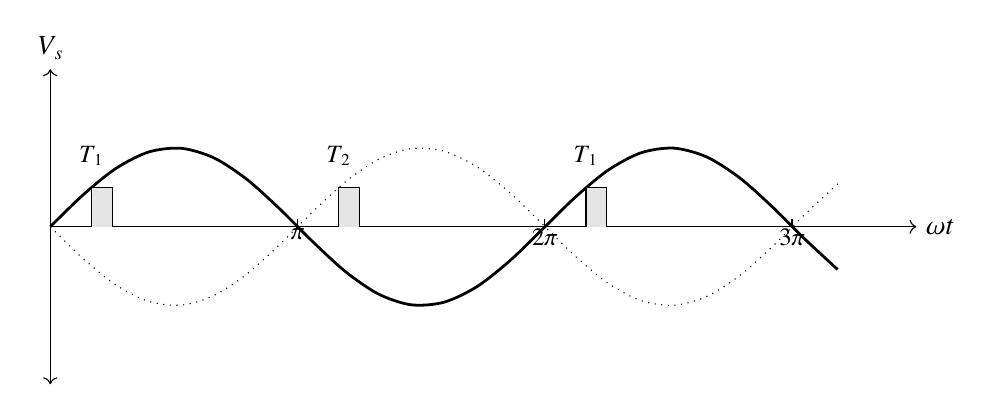
\begin{tikzpicture}[scale=1]
    \draw[->] (0,0) -- (11,0) node[right] {$\omega t$};
    \draw[<->] (0,-2) -- (0,2) node[above] {$V_s$};
    \draw[domain=0:10, smooth, variable=\x, black,line width=1pt] plot ({\x},{sin(deg(\x))});
    \draw[dotted,domain=0:10, smooth, variable=\x, black] plot ({\x},{-sin(deg(\x))});
    \foreach \x/\xtext in {3.14/\pi,6.28/2\pi,9.42/3\pi} {
        \draw (\x cm,0) -- (\x cm,0.1) node[below] {\small$\xtext$};
    }

\fill[gray!20] (0.5233,0) -- (0.5233,0.5) -- (0.785,0.5) -- (0.785,0) -- cycle;
    \fill[gray!20] (3.6633,0) -- (3.6633,0.5) -- (3.925,0.5) -- (3.925,0) -- cycle;
    \fill[gray!20] (6.8033,0) -- (6.8033,0.5) -- (7.065,0.5) -- (7.065,0) -- cycle;

    \draw (0.5233,0) -- (0.5233,0.5);
    \draw (0.5233,0.5) -- (0.785,0.5);
    \draw (0.785,0.5) -- (0.785,0);

    \draw (3.6633,0) -- (3.6633,0.5);
    \draw (3.6633,0.5) -- (3.925,0.5);
    \draw (3.925,0.5) -- (3.925,0);

    \draw (6.8033,0) -- (6.8033,0.5);
    \draw (6.8033,0.5) -- (7.065,0.5);
    \draw (7.065,0.5) -- (7.065,0);


     \node at (0.5233,0.9) {\small$T_1$};
     \node at (3.6633,0.9) {\small$T_2$};
     \node at (6.8033,0.9) {\small$T_1$};
\end{tikzpicture}
\end{figure}
\begin{figure}[!h]
    \centering
    \begin{tikzpicture}[scale=1]
    \draw[->] (0,0) -- (11,0) node[right] {$\omega t$};
    \draw[<->] (0,-2) -- (0,2) node[above] {$V_o$};
    \draw[domain=0.5233:3.14, smooth, variable=\x, black,line width=1pt] plot ({\x},{sin(deg(\x))});
    \draw[domain=3.6633:6.28, smooth, variable=\x, black,line width=1pt] plot ({\x},{-sin(deg(\x))});
    \draw[domain=6.8033:9.42, smooth, variable=\x, black,line width=1pt] plot ({\x},{sin(deg(\x))});

    \foreach \x/\xtext in {0.5233/\alpha, 3.14/\pi,4/\pi + \alpha ,6.28/2\pi,7.2/2\pi + \alpha,9.42/3\pi}{
        \draw (\x cm,0) -- (\x cm,0) node[below] {\small $\xtext$};
    }

     \draw [line width=1pt](0,0)--(0.5233,0);
    \draw [line width=1pt](0.5233,0) -- (0.5233,0.5);
    \draw[line width=1pt](3.14,0)-- (3.6633,0);
    \draw[line width=1pt] (3.6633,0) -- (3.6633,0.5);
    \draw [line width=1pt](6.28,0)--(6.8033,0);
    \draw [line width=1pt](6.8033,0) -- (6.8033,0.5);

    \node at (0.25,0.6){\small$T_2$};
    \node at (0.25,0.2){\small$D_2$};
     \node at (3.4,0.6){\small$T_1$};
    \node at (3.4,0.2){\small$D_1$};
    \node at (6.4,0.6){\small$T_2$};
    \node at (6.4,0.2){\small$D_2$};

    \node at (1.57,0.4){\small $T_1D_2$};
    \node at (4.71,0.4){\small $T_2D_1$};
    
\end{tikzpicture}
\end{figure}
\begin{figure}[!h]
    \centering
    \begin{tikzpicture}[scale=1]
    \draw[->] (0,0) -- (11,0) node[right] {$\omega t$};
    \draw[<->] (0,-2) -- (0,2) node[above] {$i_{T_1}$};
   
    \foreach \x/\xtext in {0.5233/\alpha,4/\pi + \alpha,7.2/2\pi + \alpha,10/3\pi + \alpha}{
        \draw (\x cm,0) -- (\x cm,0) node[below] {\small $\xtext$};
    }
     \draw [line width=1pt](0,0)--(0.5233,0);
    \draw [line width=1pt](0.5233,0) -- (0.5233,1);
    \draw[line width=1pt](0.5233,1)-- (3.6633,1);
    \draw[line width=1pt] (3.6633,1) -- (3.6633,0);
    \draw[line width=1pt] (3.6633,0) -- (6.8033,0);
    \draw [line width=1pt](6.8033,0)--(6.8033,1);
    \draw [line width=1pt](6.8033,1) -- (9.948,1);
     \draw [line width=1pt] (9.948,1) -- (9.948,0);

     \draw[dotted,domain=0:10, smooth, variable=\x, black] plot ({\x},{1});
     \node at (0.4,1.2) {\small $I_{DC}$};
\end{tikzpicture}
\end{figure}
\begin{figure}[!h]
    \centering
    \begin{tikzpicture}[scale=1]
    \draw[->] (0,0) -- (11,0) node[right] {$\omega t$};
    \draw[<->] (0,-2) -- (0,2) node[above] {$i_{s}$};
   

    \draw [line width=1pt](0.5233,0) -- (0.5233,1);
    \draw[line width=1pt](0.5233,1)-- (3.14,1);
    \draw[line width=1pt](3.14,1)-- (3.14,0);
    \draw[line width=1pt] (3.14,0) -- (3.6633,0);
    \draw[line width=1pt] (3.6633,0) -- (3.6633,-1);
    \draw[line width=1pt] (3.6633,-1) -- (6.28,-1);
    \draw[line width=1pt]  (6.28,-1) -- (6.28,0);
    \draw[line width=1pt] (6.28,0) -- (6.8033,0);
    \draw [line width=1pt](6.8033,0)--(6.8033,1);
    \draw [line width=1pt](6.8033,1) -- (9.42,1);
     \draw [line width=1pt] (9.42,1) -- (9.42,0);
     \draw [line width=1pt] (9.42,0) -- (9.948,0);

     \draw[dotted,domain=0:10, smooth, variable=\x, black] plot ({\x},{1});
     \node at (0.4,1.2) {\small $I_{DC}$};
    
\end{tikzpicture}
\end{figure}

From \tabref{tab:inputs.EE.59.2022}:
\begin{align}
   (I_{s_1})_{peak} &= \frac{4I_{dc}}{\pi}\cos{\left(\frac{\alpha}{2}\right)}\\
    &= \frac{4 \times 15 }{\pi}\times \cos{\frac{45 \degree}{2}}\\
    &=17.64 A 
\end{align}

%\end{document}

\pagebreak

\end{enumerate}
